% !TeX root = ./diss.tex

\documentclass[12pt,notitlepage]{report}

\usepackage{a4}
\usepackage{verbatim}
\usepackage[utf8]{inputenc}
\usepackage[british,UKenglish]{babel}
\usepackage{enumitem}
\usepackage{parskip}
\usepackage{biblatex}
\usepackage{float}
\usepackage{placeins}
\usepackage{csquotes}
\usepackage{listings}
\usepackage{dirtree}
\usepackage{float}
\usepackage{caption}
\usepackage{subcaption}
\usepackage[binary-units=true]{siunitx}
\usepackage[final]{pdfpages}
\usepackage{amsmath}
\usepackage{xcolor}
\usepackage{fancyhdr}
\usepackage[raggedright]{titlesec}
\usepackage[a4paper,left=2cm,right=2cm,top=2.5cm,bottom=2cm]{geometry}% margins
\usepackage{hyperref}
\usepackage{cleveref}

\addbibresource{refs.bib}
\defbibheading{secbib}[\bibname]{%
  \chapter*{References}%
  \markboth{#1}{#1}}

\titleformat{\chapter}[hang]    % Chapter number and name on one line
{\normalfont\huge\bfseries}{\chaptertitlename\ \thechapter:}{1em}{}
\titlespacing*{\chapter}{0pt}{0pt}{6pt}

\setcounter{secnumdepth}{4}     % subsubsections (H3) enumerated
\setcounter{tocdepth}{4}        % subsubsections (H3) in table of contents

% Fancy section referencing
\crefformat{section}{\S#2#1#3}
\crefformat{subsection}{\S#2#1#3}
\crefformat{subsubsection}{\S#2#1#3}
\crefrangeformat{section}{\S\S#3#1#4 to~#5#2#6}
\crefmultiformat{section}{\S\S#2#1#3}{ and~#2#1#3}{, #2#1#3}{ and~#2#1#3}

\definecolor{darkorange}{rgb}{0.82, 0.41, 0.12}
\definecolor{darkblue}{rgb}{0.0, 0.28, 0.67}

\DeclareSIUnit{\bits}{bits}
\DeclareSIUnit{\cycle}{/ cycle}
\DeclareSIUnit{\cycles}{cycles}
\sisetup{group-separator = {,}}

\newcommand{\candidate}{2398E}

\lstset{
  basicstyle=\ttfamily
}

\raggedbottom                           % try to avoid widows and orphans
\sloppy
\clubpenalty1000%
\widowpenalty1000%

\renewcommand{\baselinestretch}{1.1}    % adjust line spacing to make
                                        % more readable

\begin{document}

%\bibliographystyle{plain}


%%%%%%%%%%%%%%%%%%%%%%%%%%%%%%%%%%%%%%%%%%%%%%%%%%%%%%%%%%%%%%%%%%%%%%%%
% Title


\pagestyle{empty}

\hfill{\LARGE \bf Benjamin Marshall}

\vspace*{60mm}
\begin{center}
\Huge
{\bf Parallelising Sequence Alignment} \\
\vspace*{5mm}
\LARGE
Computer Science Tripos -- Part II \\
\vspace*{5mm}
Sidney Sussex College \\
\vspace*{5mm}
2020  % today's date
\end{center}

\newpage

\pagestyle{plain}
\pagenumbering{arabic}
\setcounter{page}{2}

\section*{Declaration}

I, Benjamin Marshall of Sidney Sussex College, being a candidate for Part II of
the Computer Science Tripos, hereby declare that this dissertation and the work
described in it are my own work, unaided except as may be specified below, and
that the dissertation does not contain material that has already been used to
any substantial extent for a comparable purpose.

I, Benjamin Marshall of Sidney Sussex College, am content for my dissertation to
be made available to the students and staff of the University.

\bigskip
\leftline{Signed}

\medskip
\leftline{Date \today}

\section*{Acknowledgements}

I would like to thank my supervisor Peter Rugg for his guidance and feedback throughout the project, and my Director of Studies Matthew Ireland for his feedback on this dissertation.

\newpage

%%%%%%%%%%%%%%%%%%%%%%%%%%%%%%%%%%%%%%%%%%%%%%%%%%%%%%%%%%%%%%%%%%%%%%%%%%%%%%
% Proforma, table of contents and list of figures

\chapter*{Proforma}

{\large
\begin{tabular}{ll}
Candidate Number:   & \bf \candidate                              \\
Project Title:      & \bf Parallelising Sequence Alignment        \\
Examination:        & \bf Computer Science Tripos -- Part II      \\
Examination Year:   & \bf 2020                                    \\
Word Count:         & \bf 11,945\footnotemark[1]                    \\
Line Count:         & \bf 5,172\footnotemark[2]                    \\
Project Originator: & Mr P.~Rugg                    \\
Supervisor:         & Mr P.~Rugg                    \\
\end{tabular}
}
\footnotetext[1]{
  This word count was computed by
  \lstinline{detex -l chapters/*.tex | tr -cd '0-9A-Za-z \\n' | wc -w}
}
\stepcounter{footnote}
\footnotetext[2]{
  This line count was computed using \lstinline{cloc --exclude-dir=quartus}; it excludes comments and blank lines.
}
\stepcounter{footnote}


\section*{Original Aims of the Project}

To implement the Smith-Waterman algorithm for sequence alignment in single-threaded C, multi-threaded C, and CUDA, and to thoroughly evaluate their performance.
One extension was to modify the C implementation to use Streaming SIMD Extensions to parallelise that program further.
The other extension was to implement the Smith-Waterman algorithm in SystemVerilog and instantiate it on an FPGA.
Each implementation was to utilise a variety of alignment-scoring approaches.

\section*{Work Completed}

The Smith-Waterman algorithm was implemented in single-threaded C, multi-threaded C, and CUDA (satisfying the core success criteria), and also in SystemVerilog.
The SystemVerilog implementation is limited to smaller sequences than the C and CUDA implementations.
Their performance was compared against each other, and across different alignment-scoring metrics as well.

\section*{Special Difficulties}

None.

\newpage

\tableofcontents

% \listoffigures

\newpage

%%%%%%%%%%%%%%%%%%%%%%%%%%%%%%%%%%%%%%%%%%%%%%%%%%%%%%%%%%%%%%%%%%%%%%%
% now for the chapters

\pagestyle{fancy}
\renewcommand{\sectionmark}[1]{\markright{\textsl{\MakeUppercase{\thesection.\ #1}}}}
\lhead{\rightmark}
\rhead{}
\cfoot{\thepage}
\renewcommand{\headrulewidth}{0pt}

% !TeX root = ../diss.tex

\chapter{Introduction}
The Smith-Waterman (SW) algorithm is used by bioinformaticians to find similarities between DNA or protein structures.
I implemented this algorithm using three different processor architectures: CPUs, GPUs, and FPGAs.
All of these architectures allow for parallel computation but lend themselves to extracting parallelism from the algorithm in different ways.
This dissertation discusses the relative strengths and weaknesses of these different architectures to implement this algorithm, and the varying approaches required for these different platforms.

\section{Motivation}
Sequence alignment involves finding the sections of two sequences that are most similar to one another, and recording how they differ.
This can be useful when comparing genes or proteins between species, or when identifying genetic variations or diseases between individuals of a species.
In the context of bioinformatics, sequences of amino acids make up proteins, which perform a multitude of biological functions, and sequences of nucleotides make up DNA which encodes for the construction of these proteins and controls their usage.

There is a vast quantity of sequenced protein and DNA data available, for example the GRC’s most recent human genome assembly contains over 3.1 billion base pairs \cite{GRCh38}.
Attempting to find patterns is simply intractable for humans, and sequence alignment algorithms are used instead to identify similar regions for further investigation.
This can be particularly helpful given a labelled database of sequences, such as the UniProt Knowledgebase \cite{UniProt}, a database of proteins.
Using such a database, new proteins can be aligned against database sequences to find the most similar proteins that have been previously studied, providing clues on the properties of the new protein.

\section{Previous work}
The Smith-Waterman algorithm \cite{SW_Original} is often used to align sequences, yet it is computationally expensive, requiring $O(NM)$ space and time to run in its original form, for sequences of lengths $N$ and $M$ (see \cref{sec:SW_Complexity}).
Its structure exposes a significant degree of parallelism, and there have been previous investigations into implementing it on GPUs and FPGAs for increased performance when compared to CPUs.
Investigating ways of accelerating this algorithm may lead to time and money being saved, though hardware availability is often the constraining factor in practice.
For this reason most alignments are performed on CPUs and GPUs, but it is academically interesting to explore producing a hardware accelerator nonetheless.

In this project I use and combine some previous approaches to produce implementations for each platform and compare them.
This was done several years ago by Benkrid et al. \cite{Benkrid12}, though I used more modern hardware.
This project repeats their experiment, and I investigated the impact of different scoring mechanisms on performance, which was not done by Benkrid et al.


% !TeX root = ../diss.tex

\chapter{Preparation}

There were two main areas of preparation for my project. One was to research the Smith-Waterman (SW) algorithm, and the ways it has been modified and implemented by others.
The other area was researching the different architectures, programming environment and tools to use.

\section{Overview of the Smith-Waterman algorithm}
\label{sec:SW_Overview}
Sequence alignment algorithms are used to find similar regions between two strings.
This involves predicting where symbols in the two strings correlate with each other (both matching and mismatching symbols), or where one sequence has some symbols that have been inserted into that sequence or deleted from the other.
This can be represented as follows, where symbols in the same column correspond to one another, and dashes represent insertions or deletions (gaps):
\begin{center}
\begin{tabular}{c}
\begin{lstlisting}[basicstyle=\ttfamily\linespread{0.8}]
AC-T
ACGT
\end{lstlisting}
\end{tabular}
\end{center}

The Smith-Waterman algorithm \cite{SW_Original} is a local alignment algorithm; it can produce alignments that span a subset of the input sequences.
This is useful when aligning long segments of DNA which contain non-coding regions or multiple different genes (which occurs when aligning against an entire chromosome).
When aligning a single gene against a chromosome from a different species, a local alignment algorithm can find the relevant region whilst excluding the rest of the longer sequence in the alignment.

\subsection{The Dynamic Programming approach}
\label{sec:SW_DP}

The Smith-Waterman algorithm \cite{SW_Original} finds alignments using dynamic programming.
For sequences $A=a_1 a_2 \ldots a_N$ and $B=b_1 b_2 \ldots b_M$, a scoring matrix $H$ is constructed where cell $H_{i,j}$ gives the score of the best local alignment that ends with $a_i$ and $b_j$.
Using a similarity function $s(a,b)$ which gives the similarity of two sequence symbols, and gap score list $W_k$ which gives the penalty for a deletion of length $k$, $H_{i,j}$ is defined as follows:
$$ H_{i,j} = \max \begin{cases}
H_{i-1,j-1} + s(a_i, b_j) & \text{(Including both symbols in alignment)} \\
\max_{k \geq 1}(H_{i-k,j} - W_k) & \text{(Skipping $k$ symbols from $a$)} \\
\max_{l \geq 1}(H_{i,j-l} - W_l) & \text{(Skipping $k$ symbols from $b$)} \\
0 & \text{(Starting alignment here)}
\end{cases}$$

The grid is initialised using $\forall i\leq N . H_{i,0}=0$ and $\forall j \leq M . H_{0,j}=0$.

For example, using sequences {\ttfamily GACT} and {\ttfamily ACGT} and the following definitions of $s(a,b)$ and $W_k$:
$$s(a, b)= \begin{cases}
5 &  a = b \\
-4 & a \neq b
\end{cases}
\qquad \qquad \qquad W_k = -k
$$

\begin{center}
$H = $ \begin{tabular}{|c|ccccc|} \hline
& & {\ttfamily A} & {\ttfamily C} & {\ttfamily G} & {\ttfamily T} \\ \hline
& $0$ & $0$ & $0$ & $0$ & $0$ \\
{\ttfamily G} & $0$ & $0$ & $0$ & $3$ & $2$ \\
{\ttfamily A} & $0$ & $3$ & $2$ & $2$ & ${\color{darkorange} 1}$ \\
{\ttfamily C} & $0$ & $2$ & ${\color{darkblue}6}$ & $5$ & $4$ \\
{\ttfamily T} & $0$ & $1$ & $5$ & $4$ & $8$ \\ \hline
\end{tabular}
\end{center}

Taking two examples from this:
\begin{align*}
{\color{darkblue}H_{3,2}} = 6 &= \max \begin{cases}
    3 + s(\text{\ttfamily C}, \text{\ttfamily C}) =6\\
    \max(2-1, 0 - 2, 0-3) =1 \\
    \max(2-1, 0 - 2) =1\\
    0
\end{cases} \\
{\color{darkorange} H_{2,4}} = 1 &= \max \begin{cases}
    3 + s(\text{\ttfamily A}, \text{\ttfamily T}) =1 \\
    \max(2-1, 0 - 2) =1 \\
    \max(2-1, 2 - 2, 3-3, 0-4) =1 \\
    0
\end{cases}
\end{align*}
Note that in the case of $H_{2,4}$ (and others) there are multiple ways of getting to the maximum value (from above, the left, or diagonally in this case), and this leads to multiple alignments that have the same optimal score.

\subsection{Back-tracing}
\label{sec:SW_Back_tracing}
Stored with each grid cell is a ``pointer'' which locates the previous cell in the alignment ending with that cell, where pointer $p \in \{Above_k, Left_k, Diagonal, Nil\}$. $Nil$ represents this cell not being part of an alignment, because all paths to that cell are worse than the threshold $0$. $Left_k$ represents skipping $k$ symbols from $a$, likewise for $Above_k$ skipping $k$ symbols from $b$. In the general case, this matrix of pointers $P$ is found using:
$$ P_{i,j} = \begin{cases}
    Diagonal, & H_{i,j} = H_{i-1,j-1} + s(a_i, b_j) \\
    Left_k, & H_{i,j} = \max_{k \geq 1}(H_{i-k,j} - W_k) \\
    Above_k, & H_{i,j} = \max_{l \geq 1}(H_{i,j-l} - W_l) \\
    Nil, & H_{i,j} = 0
\end{cases}$$
\pagebreak

An example of $P_{i,j}$ is as follows (where $\cdot$ represents $Nil$):
\begin{center}
$P = $     \begin{tabular}{|p{0.035\textwidth}|p{0.035\textwidth}p{0.035\textwidth}p{0.035\textwidth}p{0.035\textwidth}p{0.035\textwidth}|} \hline
& & \hfil {\ttfamily A} & \hfil {\ttfamily C} & \hfil {\ttfamily G} & \hfil {\ttfamily T} \\ \hline
& \hfil $\cdot$ & \hfil $\cdot$ & \hfil $\cdot$ & \hfil $\cdot$ & \hfil $\cdot$ \\
\hfil {\ttfamily G} & \hfil ${\color{darkorange} \cdot}$ & \hfil $\cdot$ & \hfil $\cdot$ & \hfil $\nwarrow$ & \hfil $\leftarrow_1$ \\
\hfil {\ttfamily A} & \hfil $\cdot$ & \hfil ${\color{darkorange} \nwarrow}$ & \hfil $\leftarrow_1$ & \hfil $\uparrow_1$ & $\leftarrow_1$ \\
\hfil {\ttfamily C} & \hfil $\cdot$ & \hfil $\uparrow_1$ & \hfil ${\color{darkorange} \nwarrow}$ & \hfil ${\color{darkorange} \leftarrow_1}$ & $\leftarrow_2$ \\
\hfil {\ttfamily T} & \hfil $\cdot$ & \hfil $\uparrow_2$ & \hfil $\nwarrow$ & \hfil $\leftarrow_1$ & \hfil ${\color{darkorange} \nwarrow}$ \\ \hline
\end{tabular}
\end{center}

A running maximum score is maintained during the production of the grid, and the cell $H_{i,j}$ with the highest score corresponds to the highest-scoring alignment, which finishes with $a_i$ and $b_j$.
Starting here, the alignment can be found from end to start by following the pointers in the grid. The best path through $P_{i,j}$ is highlighted in {\color{darkorange}orange}, and gives alignment:
\begin{center}
\begin{tabular}{c}
\begin{lstlisting}[basicstyle=\ttfamily\linespread{0.8}]
AC-T
ACGT
\end{lstlisting}
\end{tabular}
\end{center}

\subsection{Algorithmic complexity}
\label{sec:SW_Complexity}
For sequences of lengths $N$ and $M$, this algorithm requires $O(NM)$ space to store the two matrices, each with $(N+1)\times(M+1)$ elements.
The runtime is $O(N^2 M)$, where without loss of generality $N\geq M$.
Each cell needs to consider the cell to its diagonal (constant time), and all of the cells above it (of order $M$ cells), and all cells to its left (of order $N$ cells).
This gives a runtime for evaluating a cell as $O(N+M)$, which is $O(N)$ given $N\geq M$.
There are $NM$ cells to be evaluated, so producing the grid takes $O(N^2 M)$ time.

If the gap evaluation scheme did not maximise over a row, and instead performed constant time operations, then the complexity is $O(NM)$.
This is discussed in \cref{sec:SW_gaps}.

Each back-tracing step requires constant time (a matrix lookup, and some pointer comparisons) to produce each element in the alignment, and the length of alignment is bounded by $N+M$, where the alignment is wholly made up of gaps.
Therefore, this step requires $O(N)$ space and time, where $N\geq M$.

Overall, the space requirements of the algorithm as presented is $O(NM)$, and the time requirements are either $O(NM)$ or $O(N^2 M)$ depending on how gaps are evaluated.
Improvements to this are discussed in \cref{sec:SW_Linear_Prep}.

\subsection{Scoring alignments}
\label{sec:SW_Scoring}

The general approach to scoring alignments is given in the paper written by Smith and Waterman \cite{SW_Original}, but the exact details are not specified.
There are two areas that need definition: how to compare a pair of sequence symbols, and how to score gaps in the alignment.

\subsubsection{Sequence similarity functions}
\label{sec:SW_similarity_functions}
The original paper requires similarity function $s(a,b)$ which gives the similarity of two sequence symbols. One simple implementation might be:
$$s(a, b) = \begin{cases}
m,   & a =    b \\
\mu, & a \neq b
\end{cases}$$

For two constants $m$ and $\mu$ where typically $m>0$ and $\mu<0$.
The implementation Smith-Waterman in the European Molecular Biology Open Software Suite (EMBOSS) \cite{EMBOSS} uses an approach equivalent to using $m=5$ and $\mu=-4$ for DNA alignments by default.

However, the biological processes that leads to one symbol being substituted for another cannot be entirely expressed in these two constants, especially when some symbols are more likely than others to replace a given symbol.
This is particularly problematic in proteins, which naturally are made up of 22 different types of amino acids.

A more granular approach is to base $s(a,b)$ on a substitution matrix, which encodes a score for each different pairing of symbols.
This has performance penalties (\cref{sec:C_scoring_eval,sec:CUDA_scoring_eval,sec:SV_expected_v_actual,sec:FPGA_utilisation,sec:SV_Fmax}), because the first approach can use direct equality testing and hard-coded constants, whereas using a substitution matrix for proteins requires a lookup from a $22\times22$ matrix.

Discussions of which substitution matrices are best for which applications are beyond the scope of this project, and they are all implemented in the same way.
I chose to base investigations into the performance implications into this on the BLOSUM50 matrix for proteins \cite{BLOSUM}, which is used for alignments between sequences that are not closely related.

\subsubsection{Scoring gaps}
\label{sec:SW_gaps}
The original paper \cite{SW_Original} references a gap weight vector $W_k$, which defines the score penalty of a gap of length $k$, where gaps jump either $k$ elements to the left, or above.
However, it makes the algorithm run in $O(N^2 M)$ time for $N\geq M$ (\cref{sec:SW_Complexity}), so other approaches are used instead.

One solution to this problem was suggested by Waterman and Smith \cite{SW_Metrics} in an earlier paper about global alignment: to define $W_k=kw_1$ for some gap penalty $w_1$.
Using the recursive definition of $H_{i,j}$ the score using a $Left$ gap is:
$$\max_{k \geq 1}(H_{i-k,j} -W_k) = H_{i-1,j} - w_1$$
Gotoh proposed a different way of solving this problem \cite{Gotoh}.
The constant gap penalty models the cost of inserting or deleting symbols in a sequence by making this penalty proportional to the length of the insertion or deletion.
This is not ideal, because as Gotoh observes, ``long gap[s] can be produced by a single mutational event''.
Instead he proposes what is later called the affine-gap method, where $W_k=uk+v$ for some gap penalties $u$ and $v$.
The penalty of starting to insert or delete a sequence is given by $u$, and $v$ accounts for the different lengths of such a sequence.

This approach requires more space than the original Smith-Waterman algorithm because choosing whether to open a gap has an impact on scores later in the alignment.
When evaluating a mismatched cell in the dynamic-programming grid it is impossible to know whether to pay the mismatch penalty because a sequence of matches immediately follow, or if a long sequence of mismatches follow and it would be less expensive to open up a gap to cover them instead.
Therefore, extra space is needed to keep track of scores when the decision to open a gap is and also is not taken.

To achieve this, three grids are constructed instead of one.
This triples the memory requirements in practice but does not change the asymptotic memory requirements.
The main score grid $H_{i,j}$ is calculated using a similar approach to before, representing the score of the best alignment using sequences $a_1\ldots a_i$ and $b_1 \ldots b_j$.
Additionally, there is grid $F_{i,j}$ which represents the score of the best alignment between $a_1\ldots a_i$ and $b_1 \ldots b_j$ provided it ended with an open left-gap.
$G_{i,j}$ is similar for above gaps.
This gives grid definitions:
\begin{align*}
H_{i,j} &= \max(H_{i-1,j-1} + s(a_i, b_j), F_{i,j}, G_{i,j}, 0) \\
F_{i,j} &= \max(H_{i-1,j} + u + v, F_{i-1,j} + v) \\
G_{i,j} &= \max(H_{i,j-1} + u + v, G_{i,j-1} + v)
\end{align*}

This is modified from the original paper somewhat for notational consistency with the rest of the dissertation.

Pointer grids need to be stored for all three grids, where the back-tracer will start in grid $H$ (and this is the only grid where the running maximum is kept), but it will trace through $F$ and $G$ as well to determine where a gap started.

\subsection{Linear space modification to Smith-Waterman algorithm}
\label{sec:SW_Linear_Prep}
\subsubsection{Overview}
\label{sec:SW_Linear_Overview}

A common approach to improving the runtime of the Smith-Waterman algorithm is to reduce the amount of space used by increasing the amount of time spent in doing arithmetic.
Hirschberg’s algorithm \cite{Hirschberg} pioneered this approach for the Longest Common Subsequence problem.
Myers and Miller apply this approach to local alignments \cite{MyersMiller}, which is summarised below.

The purpose of this algorithm is to correctly and efficiently split the alignment into small chunks, manageable for the quadratic space implementation which is where the back-tracing is done.
It recursively divides a large grid into two smaller grids.
\Cref{fig:Linear_Space_Structure} shows this, where the optimal alignment is shown in orange.
The grid has been divided into two smaller grids by the first pass of the algorithm, a grid with blocks $1$ and $2$, and the grid with blocks $3$ and $4$.
The grey segments do not contain the alignment and can be ignored.
The black arrows represent the direction the blocks are evaluated in, discussed further on.

\Cref{lst:pseudo_sw} is a pseudo-code representation of the quadratic space Smith-Waterman algorithm, to be used in this linear space algorithm.
Parameter \lstinline{fixedTop} specifies whether the alignment can start from anywhere in the grid, or just the top left corner (and is implemented by including or removing the options of $0$ and $Nil$ from the maximising functions).
This is necessary because the optimal alignment inside a subproblem may not start at the top-left, but the overall optimal alignment may pass through multiple sub-grids where the top-left of each grid must be connected to the bottom-right of the next grid.
Parameter \lstinline{fixedBottom} is similar, specifying whether to start back-tracing at the best cell in the grid, or the bottom-right cell.

\begin{figure}
    \centering
    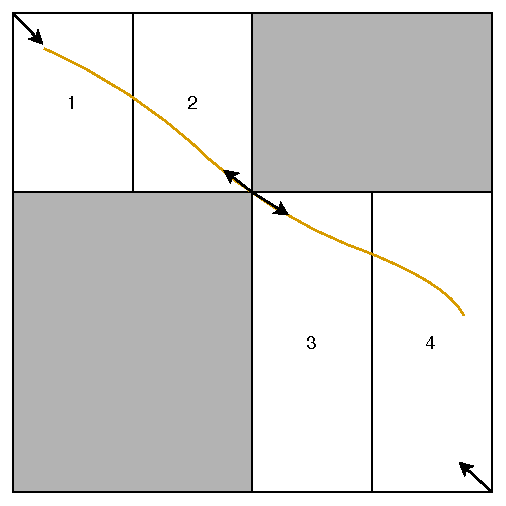
\includegraphics[width=(0.4\textwidth)]{figs/linear_space_structure.pdf}
    \caption{The divided dynamic programming matrix when using the linear space approach, after the first iteration}
    \label{fig:Linear_Space_Structure}
\end{figure}

\begin{lstlisting}[basicstyle=\linespread{0.9}\ttfamily\footnotesize, label={lst:pseudo_sw},captionpos=b,caption={Pseudo-code representation of quadratic space implementation of SW algorithm}]
fun sw(seq1, seq2, fixedTop, fixedBottom):
    Dynamic programming approach using quadratic space
    if fixedTop:
        Only allow alignments to start at the top-left
    else:
        Allow alignments to start anywhere
    if fixedBottom:
        Return the alignment ending at the bottom-right grid cell
    else:
        Return the alignment ending at the best cell in the grid
\end{lstlisting}

To split a large grid into two smaller grids, the scores of the middle column of cells are found by starting from the top-left and working towards the middle, and also by starting from the bottom right and working towards the middle.
\Cref{lst:pseudo_sw_col} is a representation of this.
In \cref{fig:Linear_Space_Structure}, blocks $1$ and $3$ are evaluated from their top-lefts to their middle columns, and blocks $2$ and $4$ from the bottom-right, and the direction of evaluation represented by the black arrows.
These scores are found using a linear space.
These two columns are added together, and each cell of the column gives the score for the best alignment that passes through that cell.
The optimal alignment might cross the middle column or be in one of these half-grids.

The middle columns are found using $O(N)$ space for sequences of lengths $N$ and $M$, and maintains $O(NM)$ time complexity, albeit with a greater constant factor.
This uses the fact that only the immediate neighbours are needed to calculate the score of a cell, so the values of a previous column can be discarded once the values in the next column have been computed. This data dependency is shown in \cref{fig:Linear_Space_Dependencies}.
However, discarding this information leads to recomputation of the cells in the smaller subproblems that are recursively evaluated.

Maxima are calculated whilst computing each half, and compared to the maximum cell in the summed columns.
If the overall maximum is in one of the half-grids, restart the algorithm between that cell and the top-left or bottom-right, if on the left or right sides respectively.
Otherwise, the algorithm is rerun between the end cells and the maximum middle cell.
This recursively breaks up the alignment until it is small enough to tackle directly using the quadratic space algorithm (\cref{sec:SW_DP,sec:SW_Back_tracing,sec:SW_Complexity}), and then joins them back together.
\begin{figure}[h]
    \centering
    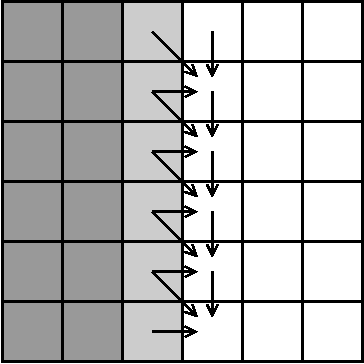
\includegraphics[width=(0.4\textwidth)]{figs/linear_space_deps.pdf}
    \caption{Data dependencies when using the linear space approach}
    \label{fig:Linear_Space_Dependencies}
\end{figure}
\begin{lstlisting}[basicstyle=\ttfamily\linespread{0.9}\footnotesize, label={lst:pseudo_sw_col},captionpos=b,caption={Pseudo-code representation of linear space algorithm which finds middle columns}]
    fun sw_col(seq1, seq2, direction, fixedStart):
        direction in {forwards, backwards}
        direction determines which half of grid is evaluated
            - Forwards: from top left, to column (seq2/2)
            - Backwards: from bottom right, to column (seq2/2)
        fixedStart similar to fixedTop of sw()
        Calculate grid column by column, returning:
            - Values of column (seq2/2)
            - Location of best cell, and score
    \end{lstlisting}
\begin{minipage}{\linewidth}
\begin{lstlisting}[basicstyle=\linespread{0.9}\ttfamily\footnotesize, label={lst:pseudo_sw_linear},captionpos=b,caption={Pseudo-code representation of the linear space Smith-Waterman algorithm}]
fun sw_linear(seq1, seq2, fixedTop, fixedBottom):
    if seq1 and seq2 are small:
        return sw(seq1, seq2, fixedTop, fixedBottom)
    else:
        (forwardCol, bestForwards) = sw_col(seq1, seq2, forwards, fixedTop)
        (backwardCol, bestBackwards) = sw_col(seq1, seq2,
                                              backwards, fixedBottom)
        middleCol = forwardCol + backwardCol # Using vector addition
        bestMiddle = max(middleCol)

        # Using list splicing: seq1[x:] = [seq1[x], seq1[x+1], ... seq1[n]]
        if best path is bottom-right to bestBackwards and not fixedTop:
            return sw_linear(seq1[bestForwards.i:], seq2[bestForwards.j:],
                             fixedTop, fixedBottom)
        else if best path is top-left to bestForwards and not fixedBottom:
            return sw_linear(seq1[0:bestForwards.i], seq2[0:bestForwards.j],
                             fixedTop, fixedBottom)
        else use middle cell:
            alignStart = sw_linear(seq1[0:bestMiddle.i],seq2[0:len(seq2/2)],
                                   fixedTop, true)
            alignEnd = sw_linear(seq1[bestMiddle.i:],seq2[len(seq2/2):],
                                 true, fixedBottom)
            return alignStart @ alignEnd
\end{lstlisting}
\end{minipage}

\subsubsection{Back-tracing}
\label{sec:SW_Linear_Back_tracing}

The process of building the final alignment, back-tracing, is done in parts and later joined, in accordance with the divide-and-conquer approach of this algorithm.
When the large grid has been recursively divided to small enough grids, the quadratic space algorithm (\cref{sec:SW_DP,sec:SW_Back_tracing}) is used to find an alignment.
This is because producing an alignment requires a grid of pointers taking $O(NM)$ space, so when the grid is small enough for a full grid of pointers to be made, a full grid of scores can also be made.
The resulting aligned sequences from each of these small alignments can be joined together to make the overall alignment.

\subsubsection{Runtime complexity}
\label{sec:SW_Linear_Complexity}
This additional arithmetic does not impact the runtime complexity.
For sequences of lengths $N$ and $M$ the linear space approach evaluates $2NM$ grid cells (each taking $O(1)$ time).

The amount of work done in each iteration halves. The first step evaluates every grid cell, taking $NM$ evaluations (over two halves of size $\frac{N}{2} \times M$).
If the alignment is in one half, then the next area to evaluate has at least halved.
If the alignment is split across the middle column, some point at position $m$ will be chosen on that column.
Then two grids will be evaluated of area $\frac{N}{2} \times m$ and $\frac{N}{2} \times (M-m)$ which sum to $\frac{NM}{2}$ for all possible $m$.
Using this repeated halving of work, the total number of grid evaluations required is:
$$ \text{Cells evaluated } =  NM + \frac{NM}{2} + \frac{NM}{4} + \cdots \leq NM \sum_{i=0}^\infty 2^{-i} = 2NM $$

\section{Overview of architectures and programming languages used}
\label{sec:Architecture_prep}
The objective of my project was to implement the Smith-Waterman algorithm using different hardware architectures (general purpose CPUs, GPUs, and FPGAs).
As part of my preparation I learnt about these architectures so I could produce implementations that were best suited for these different architectures.

\subsection{Central Processing Units and C}
\label{sec:CPU_prep}
Modern general-purpose Central Processing Units (CPUs) can have very high clock speeds, multiple processing cores, and have rich Instruction Set Architectures (ISAs).
The CPU in my laptop, used by this project, is an Intel Core i7-8750H.
This has six processing cores, and has a maximum clock frequency of $\SI{4.1}{\giga\hertz}$ \cite{i7-8750H}.
This clock frequency is significantly higher than the other platforms I used, however other implementations will be able to do more work per clock cycle, using increased parallelism or specialisation.

I chose to write my programs for the CPU in C. The major reason I chose to do so was that the GPU APIs available (CUDA and OpenCL) are APIs for C/C++, so for the sake of interoperability it made sense to implement my project in either C or C++.
This would allow me to later reuse segments of code for the GPU implementation, especially the control logic and testing framework.
Also, I had previous experience with C from Part IB and a summer internship, so I chose to use C.

The focus of my project is exploring parallelism in Smith-Waterman, and with a multicore CPU I could implement a solution that was multi-threaded.
This is not a native feature in the C language, so I used the Native POSIX Thread Library, part of the GNU C Library.
This allows multiple threads to be run on multiple processing cores, where all of the scheduling is handled by the library and the host operating system.

\subsection{Graphics Processing Units and CUDA}
\label{sec:GPU_prep}
Graphics Processing Units (GPUs) are designed to exploit vector-level parallelism in programs. The GPU in my laptop, used by this project, is an Nvidia GTX 1050 Ti.
It has $768$ CUDA cores in it \cite{1050-Ti}; it can compute up to $768$ different things in parallel.
This is much more parallelised than the CPU, though the device has a significantly lower clock speed of $\SI{1392}{\mega\hertz}$.

I chose to use CUDA, Nvidia’s proprietary API for programming their GPUs.
An alternative was OpenCL, but I chose CUDA because it has a more helpful profiling tool, which suggests possible sources of poor performance, and I used this to guide development.

The highly parallel nature of CUDA causes its execution model to be different to a single core of a CPU.
In CUDA, a body of work is a grid, which is a group of blocks, where a block is a group of threads.
The GPU has a collection of streaming multiprocessors (SMs, in my case $24$) which execute different blocks, and each of these SMs execute $32$ threads at once.
These groups of threads are called warps and are subsets of blocks.
Threads in a warp execute in lockstep, with a single instruction for all $32$ threads in the warp.
The overall number of CUDA cores is $24 \times 32=768$.

Units of code to be run on the GPU are called kernels, which are similar to C functions. When a kernel is called the number of blocks and threads in a block are specified.
There is a hard limit to the size of a block of $1024$ threads \cite{CUDA_Guide}, therefore programs implemented in CUDA cannot require synchronisation over an arbitrary number of threads.

All of the threads are given the same arguments and execute the same blocks of code (though different paths may take different branches through the code).
All that distinguishes them are two variables, their \lstinline{threadId} and \lstinline{blockId}.
All threads within a block can be synchronised using the execution barrier \lstinline{__syncthreads()}.
However, there is no synchronisation between blocks, even when executing the same kernel, and they can execute in parallel to each other.

\subsection{Field Programmable Gate Arrays and SystemVerilog}
\label{sec:FPGA_prep}
An extension to my project was to implement the Smith-Waterman algorithm on an FPGA using a hardware description language (HDL).
I chose to use SystemVerilog as my HDL, because I had studied it in Part IB.
Field Programmable Gate Arrays are programmable circuits, principally made up of programmable lookup tables, flip-flops, integrated memory blocks and programmable routing between the features on the chip.
These devices can be programmed to make custom circuitry on the FPGA chip.

This is appealing because it allows me to define a custom accelerator optimised just for this problem, able to evaluate a cell in the dynamic programming grid in just one clock cycle.
My other implementations require numerous clock cycles to do this same work.
The device is clocked significantly slower than the CPU or GPU, with the default clock frequency of my device being $\SI{50}{\mega\hertz}$, and the theoretical maximum of $\SI{550}{\mega\hertz}$.
However, being able to do more work per clock cycle can reduce the impact of a slower clock frequency.

Although an implementation on an FPGA will require much more power and be significantly slower than the same logic in an ASIC, working with an FPGA was possible for this project and manufacturing an ASIC would cost far too much money.

I used a Terasic DE1-SoC board \cite{DE1-SoC} loaned from the Computer Architecture Group.
This has an Altera Cyclone V SE FPGA SoC \cite{CycloneV}, which has $\SI{85000}{}$ logic elements; a fairly small FPGA, but also not the smallest produced. This device was significantly older than the CPU and GPU it was compared against. This FPGA uses a 28nm process and was made in 2012 \cite{CycloneV}, whereas the CPU and GPU are from 2018 and use a 14nm process \cite{i7-8750H} \cite{1050-Ti}.
A smaller process node might improve the maximum frequency of a design implemented on an FPGA, and there would be more resources on the device at a similar price, which could be used to do more work in parallel.

The FPGA SoC also has a dual-core ARM Cortex-A9 on the same package as the FPGA \cite{CycloneV}, referred to as the Hard Processing System, HPS.
The ARM core can control the accelerator using an interconnect between the HPS and FPGA.
In particular, it provides a memory-mapped Avalon streaming interface, where the HPS requests to read or write to the FPGA as if it were memory and the FPGA’s responses to these requests can be defined in HDL.

A major design consideration for my work on the FPGA was memory capacity, due to the quadratic memory requirement of the Smith-Waterman algorithm.
There are several different types of memory on the FPGA \cite{CycloneV} and development board \cite{DE1-SoC} I was using, suited for different things.
This is tabulated in \cref{tab:FPGA_Memories}.
For the SDRAM memories, the throughput given (marked \dag) is the peak throughput, but average throughput will be lower as selecting rows takes time.
The ways that these memories were used was discussed in \cref{sec:Memory_in_SV}.

\begin{table}[h]
    \centering
    \begin{tabular}{|p{0.2\textwidth}|p{0.4\textwidth}p{0.1\textwidth}p{0.2\textwidth}|} \hline
        Name & Description & Capacity & Throughput \\ \hline
        ALM Registers & On-chip; all registers are directly accessible by routing elements & $\SI{15.67}{\kibi\byte}$ & $\SI{15.67}{\kibi\byte\cycle}$  \\ \hline
        M10K Blocks & On-chip; made up of $\SI{10}{\kibi\bit}$ blocks units where $\SI{40}{\bits}$ can be accessed in a cycle, which are pipelined with one delay-slot between request and action.  & $\SI{49.63}{\kibi\byte}$ & $\SI{1.94}{\kibi\byte\cycle}$ \\ \hline
        FPGA SDRAM & Off-chip; requires additional hardware to interface with it, and multiple delay slots as rows and columns are selected. & $\SI{64}{\mebi\byte}$
         & $\SI{2}{\byte\cycle}^\dag$ \\ \hline
        HPS DDR3 & Off-chip; requires additional hardware to interface with it, and multiple delay slots as rows and columns are selected. & $\SI{1}{\gibi\byte}$ & $\SI{8}{\byte\cycle}^\dag$ \\ \hline
        \end{tabular}

    \caption{Types of memory on the Terasic DE1-SoC development board}
    \label{tab:FPGA_Memories}
\end{table}

\FloatBarrier

\subsection{Licencing}
\label{sec:Licencing_prep}

The majority of tools and libraries I used for my project are open source, and the rest are available for private use.
\begin{itemize}
\item GNU Compiler Collection; particularly the C compiler---GPLv3
\item GNU C Library, particularly Native POSIX Thread Library---LGPL
\item GNU Debugger; for C and CUDA code---GPLv3
\item Gprof; C profiler---GPLv3
\item JetBrains CLion; C IDE---student license
\item Visual Studio Code; general source-code editor---MIT License
\item CUDA Toolkit; including a compiler, debugger, memory-checking suite and profiler---proprietary, freely distributed
\item Quartus Prime Lite Edition; for simulating and synthesising HDL designs---proprietary, freely distributed
\item Git; for version control of all source code and dissertation text---GPLv2
\item LaTeX; for typesetting this dissertation---LPPL
\item BibTeX; for references in this dissertation---GPLv3
\end{itemize}

\section{Development methodology}
\label{sec:Methodology_prep}

The plan for the project was outlined in the project proposal (\cref{sec:Proposal}), sequentially implementing designs for each platform.
By doing this, if any unexpected difficulty arose in the later stages of the project, then there would still be completed implementations from earlier in the project to evaluate.
The implementations were ordered in ascending difficulty and my descending confidence, to this end, with the first three required for the core success criteria.
In order these were:
\begin{enumerate}
\item Implementing the Smith-Waterman algorithm in single-threaded C code.
\item Modifying the C code to make it multi-threaded.
\item Implementing the Smith-Waterman algorithm in CUDA.
\item Implement the Smith-Waterman algorithm in SystemVerilog and simulate design.
\item Instantiate Verilog implementation on an FPGA.
\end{enumerate}

I tested throughout development and had two main testing areas: correctness and performance. Any errors were likely to propagate between implementations where similar approaches were used, especially between C and CUDA, so it was important to catch errors as they arose instead of letting them propagate.
I used an external implementation \cite{EMBOSS} to check my first C programs.
I tested the rest of my work using this implementation, because the reference implementation would only give one correct solution when there might be more than one for a given alignment problem, whereas my programs could decide whether a given alignment was valid and optimal.

\section{Starting Point}
\label{sec:Starting_Point}

I started with reasonable experience with C, having studied it in Part IB and writing some utility programs in C during a summer job. I had no experience with CUDA, or GPU programming in general, and had written a small amount of SystemVerilog during Part IB, but never having attempted a project of this scale in it before.
Therefore, in my project plan I assigned more time for the GPU and FPGA implementations compared to the CPU implementation, based on my relative levels of experience.

The only code used that was not my own was SystemVerilog used for administrative purposes.
I used a template from the Part IB ECAD+Arch course for instantiating a SystemVerilog design on the development board I was using, which correctly arranged IO pins.
My supervisor, Peter Rugg, gave me the Verilog he had used to build an Avalon streaming interface between the HPS and the FPGA, to transfer data between my hardware design and the OS on the HPS.
I based my streaming interface on this, and I am grateful for his assistance.

Sequence alignment and Smith-Waterman in particular are covered in detail by the first few lectures of the Part II Bioinformatics course, and is presented in \cref{sec:SW_Overview}.
This course runs in Michaelmas term.
The linear space approach (\cref{sec:SW_Linear_Prep}) is described for global alignment in that course, and I read a paper \cite{MyersMiller} for its application to local alignments.


% !TeX root = ../diss.tex

\chapter{Implementation}

\section{C implementation}
\label{sec:C_impl}

\subsection{Initial implementation}
\label{sec:Initial_C_impl}

First, I implemented Smith-Waterman’s algorithm in single-threaded C code.
I started with a simple implementation that stored the entire grid in a 2D array and calculated grid cells sequentially, which involved rewriting the definitions of the Smith-Waterman algorithm in C.
An excerpt (where \lstinline{decideCellSW} is similar to a \lstinline{max} function but also returns a pointer) is \cref{lst:c_sw}.

\begin{lstlisting}[language=C,float,basicstyle=\linespread{0.9}\ttfamily\footnotesize, label={lst:c_sw},captionpos=b,caption={Excerpt from C implementation of Smith-Waterman algorithm}]
for (unsigned long i = 0; i < len1; i++) {
    for (unsigned long j = 0; j < len2; j++) {
        decisions[i+1][j+1] = decideCellSW(
                decisions[i][j].score + match(seq1[i], seq2[j]),
                decisions[i][j+1].score + GAP_PENALTY,
                decisions[i+1][j].score + GAP_PENALTY
        );
        if (decisions[i+1][j+1].score >= bestCell->score) {
            bestCell->score = decisions[i+1][j+1].score;
            bestCell->i = i+1;
            bestCell->j = j+1;
        }
    }
}
\end{lstlisting}
This simple implementation did not perform very well, especially with long strings.
It is single-threaded, and the grid takes $O(NM)$ space for sequences of lengths $N$ and $M$.
Space was a major issue; working with the large grid in RAM was costly.
The number of alignments that could be run in parallel was limited due to memory constraints.
This is quantified in \cref{sec:C_impls_eval}.
However, this quadratic space implementation was used as a component of the linear space variant, and it also was the basis of my correctness testing (\cref{sec:Correctness_eval}).

\subsubsection{Back-tracing}
\label{sec:Initial_C_back_tracing}
In this implementation, nearly all of the time was spent filling out the of the grid (\cref{sec:C_occupancy}).
After this, an alignment was produced using a process called back-tracing (\cref{sec:SW_Back_tracing}). Stored with each grid cell is a ``pointer'' which locates the previous cell in the best alignment ending with that cell.

Using these pointers, starting at the best cell in the grid, a pair of aligned sequences is built up from back to front by following the pointers upwards and leftwards to a cell with a $Nil$ pointer.
This takes as many steps as there is symbols in the alignment, and an upper bound on this is $N+M$ steps for sequences of lengths $N$ and $M$.

\subsubsection{Linear space implementation}
\label{sec:Initial_C_Linear}
This implementation was a direct implementation of the algorithm described in \cref{sec:SW_Linear_Prep}.
It was slower than the quadratic space implementation, which was unsurprising because twice as much arithmetic was involved (\cref{sec:SW_Linear_Complexity}).
However, the implementation only took $50\%$ longer due to decreased memory usage and associated memory overheads (\cref{sec:C_impls_eval}).
Due to decreased memory usage there were not issues with performing multiple alignments at the same time, and the structure of the algorithm was amenable to parallelisation.

\subsection{Multi-threaded implementation}
\label{sec:Multi_threaded_C_impl}
This linear-space algorithm (\cref{sec:SW_Linear_Prep}) was simple to parallelise, because each grid could be processed in parallel.
Memory consistency is trivial to maintain because no data is shared between running threads; threads just join after processing their grid segment.
However, given infinite threads there is still a finite speedup, because the number of different segments of the grid available for evaluation is limited.
This limit increases as the algorithm progresses.
At the start, there are two grid segments (each taking half of the whole grid) being evaluated to find their middle columns.
If the optimal alignment crosses the middle column, the algorithm is applied recursively between the chosen cell in the middle column, and the top-left or bottom-right of the rest of the grid.
This has four sub-grids (a forwards and backwards one on each side of the middle column), covering a total area of half of the grid. Assuming infinite threads, this generalises to:
$$\text{Cells evaluated } = \frac{1}{2} \times NM + \frac{1}{4} \times \frac{NM}{2} + \frac{1}{8} \times \frac{NM}{4} + \cdots \leq \frac{1}{2} \times NM \sum_{i=0}^\infty 2^{-2i} = \frac{2NM}{3}$$

This limit was not reached in practice (\cref{sec:C_impls_eval}) but it is useful to consider.
To improve on this limit, there would need multiple threads working on each segment of the grid.
A major concern with this is synchronising threads such that they only evaluate cells when the cells they depend on have been evaluated by a different thread.
This could yield poor performance due to threads waiting on each other, and for this reason I did not prioritise implementing this approach, and I did not have time to do so.
GPUs and FPGAs are attractive platforms for solving this problem because they make it very simple to schedule threads relative to one another.

\subsubsection{Synchronisation and scheduling of work}
\label{sec:Sync_and_scheduling_of_multi-threaded_C}
I used the Native POSIX Thread Library, part of the GNU C Library, to implement this multithreaded solution.
The scheduling of threads is handled by the library and the host operating system.
By assigning the work to fill out the two halves of a grid to two different threads, and also the two recursive calls of the linear space solver to different threads, the linear space algorithm is straightforward to parallelise.
This can be seen in \cref{fig:Linear_Space_Structure}, where the numbered blocks can each be evaluated by a different thread.

My implementation was slightly more complex, allowing me to investigate how the number of available CPU cores changed the throughput of my implementation.
The results of this are presented in \cref{sec:C_params_eval}.
This was achieved using a counting semaphore to represent the number of concurrent threads performing arithmetic.
This semaphore guards the regions that were evaluating grid cells, which corresponds to the \cref{lst:pseudo_sw,lst:pseudo_sw_col}.
Threads about to enter these regions wait on the semaphore, and signal the semaphore when they leave those regions.
The effect of different numbers of working threads could be evaluated by changing the size of the semaphore.
The highest throughput on my 6-core SMT CPU was achieved using 12 threads (\cref{sec:C_params_eval}).

\subsection{Sequence similarity functions and scoring gaps}
\label{sec:Scoring_in_C_impl}
The two forms of sequence similarity function discussed in \cref{sec:SW_similarity_functions} were implemented, and the performance was evaluated later (\cref{sec:C_scoring_eval}).

Both the linear and affine gap scoring mechanisms were implemented.
The linear space implementation needed to account for horizontal gaps being opened on one side of the middle column but continued through to the other side.
This can be solved by adding the middle columns coming for both the the gap matrix $P_{i,j}$ and the score matrix $H_{i,j}$.
These decisions also need to be propagated into the sub-problems as well.
This was the approach taken by Myers and Miller \cite{MyersMiller} in their adaption of Hirschberg’s algorithm \cite{Hirschberg} to local alignment.

\section{CUDA implementation}
\label{sec:CUDA_impl}
My implementation in CUDA took a similar approach to the C implementation but using a streaming multiprocessor to evaluate many grid cells in parallel on the same device.
The SIMT (single-instruction, multiple-thread) architecture makes it is easier to synchronise work between multiple threads running the same instructions.
In CUDA there are two broad categories of parallelism: parallelism between threads (parallelism inside a multiprocessor), and parallelism between blocks (parallelism between multiprocessors).
Each of these were utilised in my implementation.

\subsection{Parallelism between threads}
\label{sec:Thread_Parallelism_in_CUDA}
Multiple threads run inside of a block simultaneously, scheduled in warps of $32$ threads, with shared memory and barrier synchronisation to allow for cooperation between threads in different warps.
I built up a diagonal front of threads, so that threads only depend on results that other threads have already computed.
This is similar to the approach taken by Ling et al. \cite{Ling_GPU}, however in their approach they exploit parallelism between blocks by running multiple alignments at the same time, whereas I chose to use multiple blocks in a single alignment.
Under my design multiple different alignments can also be running in parallel, but large and difficult alignments can exploit more than one streaming multiprocessor.

Threads on the anti-diagonal to the grid have no data dependencies and can be executed in parallel.
This is the basis for much of the parallelisation in the GPU and FPGA implementations.
This can be seen in \cref{fig:Diagonalised_Grid}, where dark grey cells have already been computed, and light grey cells can all be computed in parallel.
Dependencies between cells are shown as red arrows.

\begin{figure}
  \centering
  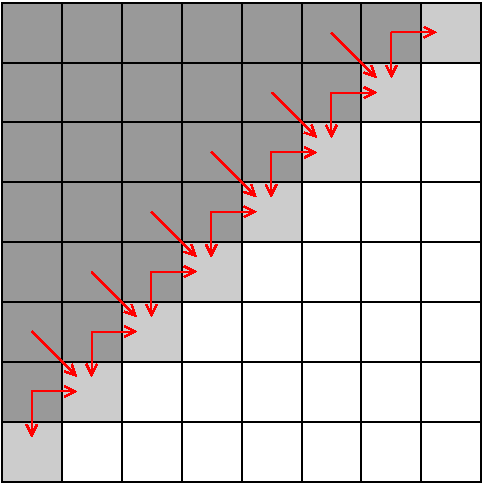
\includegraphics[width=\textwidth/2]{figs/diagonalised_grid.pdf}
  \caption{An anti-diagonal of data dependencies in Smith-Waterman’s algorithm}
  \label{fig:Diagonalised_Grid}
\end{figure}

The general approach is to assign each column to a thread and stagger the threads so that if thread $t$ is working on row $r$, then thread $t+1$ is working on row $r+1$.
Threads are then synchronised using a barrier so that only one anti-diagonal is being computed at a time.
With an unlimited number of threads, the time spent calculating the grid changes from being quadratic to linear in sequence length, taking $N + M - 1$ steps because there are that many anti-diagonals in a grid of dimensions $N\times M$.

In reality, there is a limit to the number of threads allowed in a block in CUDA ($1024$ threads), and only $32$ threads of a given block can be executing at once.
Therefore, every column cannot be assigned its own exclusive thread.
My first approach was to have a single block of threads generate the entire grid, by generating blocks of columns at a time, where each individual column had its own thread and upon reaching the end of the columns, new blocks of columns were generated.
However, when profiling my program using NVProf, it suggested that a way to improve performance might be to spread my work out over multiple thread blocks, which would spread the work over multiple streaming multiprocessors.
This had a noticeable performance improvement (\cref{sec:CUDA_single_multi_block_eval}).

\subsection{Parallelism between blocks}
\label{sec:Block_Parallelism_in_CUDA}

The opportunity for parallelism described in \cref{sec:Thread_Parallelism_in_CUDA} exists between blocks of threads, as well as threads themselves.
Although squares in \cref{fig:Diagonalised_Grid} represent threads, it also is an accurate representation when squares represent blocks as well.
This is the basis of my implementation for generating the grid using multiple blocks at once.

However, a different approach needs to be taken for communications between different anti-diagonals.
It is possible to impose an ordering of execution between threads in a block, but it is not possible to impose an ordering between blocks of a kernel grid.
There is no guarantee on the order in which blocks may be executed, there is a limit to the number of blocks that can be resident on the device, and blocks cannot leave the device until they have finished executing.
Therefore, attempting to impose an ordering by building up concurrency primitives from global memory may lead to deadlock.

Therefore, the kernel needs to be broken up into multiple smaller kernels, where blocks have no dependencies on one another.
This is done using the approach outlined above on the block-scale, where a kernel is made up of an anti-diagonal of blocks, and the number of blocks depends on the size of the grid and which anti-diagonal is being computed.
Each block writes out its right and bottom edges to global memory on the device, ready for the next block from the next kernel to consume.
All the data remains on the device so there is relatively little overhead in making many blocks for relatively short periods of time.

\subsection{Memory types}
\label{sec:Memory_in_CUDA}

The grid of scores and pointers is stored in the global memory, which is the GDDR5 VRAM used by the GPU.
There is $\SI{4}{\gibi\byte}$ of this in my laptop and it has much higher bandwidth than the DDR4 main memory in the laptop.
GPUs are designed to hide memory access latency for this memory by context switching between many different threads, so it is a good fit for this algorithm with many loads and stores.

Alternatively, shared memory (on the die of the GPU) could have been used but this is too small with only $\SI{1152}{\kibi\byte}$ available.
A block of $1024$ threads has access to only $\SI{48}{\kibi\byte}$, with room for a $78\times78$ cell grid.
With a capacity of $\SI{4}{\gibi\byte}$, the GDDR5 VRAM, was the best choice for storing the grid.

\subsection{Back-tracing}
\label{sec:Back_tracing_in_CUDA}

Back-tracing is performed on the GPU.
Even though it is a sequential process that only uses one thread of a $32$-thread multiprocessor, it is significantly quicker than it would be to copy the entire grid out of VRAM into RAM, and have the CPU run the back-tracing.
To back-trace on the CPU, too much time would be wasted copying over unwanted data: only $N+M$ grid cells could be needed out of the $N\times M$ cell grid, and finding which are needed is the process of back-tracing.

\subsection{Linear space improvements}
\label{sec:Linear_space_CUDA}

For similar reasons to the C implementation, there are performance limitations when using this quadratic space algorithm.
For large sequences memory will simply run out; a $\SI{23710}{} \times \SI{23170}{}$ grid is the largest grid that will fit in the $\SI{4}{\giga\byte}$ VRAM.
Fortunately, the linear space algorithm (\cref{sec:SW_Linear_Prep}) can also be implemented in CUDA using the same techniques discussed in \cref{sec:Thread_Parallelism_in_CUDA,sec:Block_Parallelism_in_CUDA,sec:Memory_in_CUDA,sec:Back_tracing_in_CUDA}.

Using this approach the problem is divided in half repeatedly; calculating the scores for the middle column using linear space to decide where to divide.
The control logic was implemented on the host device (the CPU), but the evaluation of grid cells and back-tracing of alignments was done on the GPU.
This was a sensible choice because most of the control flow decisions are sequential which would poorly utilise 32-thread multiprocessor on the GPU.
Moreover, the CPU achieves a much higher clock frequency and sequential throughput than the GPU.

Calculating a half-grid segment requires multiple kernel invocations for each segment, so the control logic was also multi-threaded where each segment had its own thread.
This was facilitated by CUDA Streams, which are similar to OS processes or threads.
When evaluating a grid, all of the blocks on the current anti-diagonal need to have finished before the next anti-diagonal can be processed, and the CPU can only synchronise with the GPU when either the entire GPU finishes all available work, or when all work in a stream has finished.
With each thread of C code assigned its own CUDA stream, the thread can synchronise with the work it has sent to the GPU whilst leaving other streams (and therefore threads) to utilise the GPU at the same time.
The first few and last few anti-diagonals of a grid will have fewer blocks of work than streaming multiprocessors available, so utilisation of these multiprocessors can be increased by using multiple concurrent streams of work, working on different parts of the alignment.

Using this implementation to compare multiple sequences at once is trivial, simply a new thread and stream is created for each alignment, and all subsequent new threads and streams required will be created by the alignment program.
All scheduling is done by the operating system and GPU hardware, which should lead to maximum resource utilisation provided there is the work to consume it.

\subsection{Sequence similarity functions and scoring gaps}
\label{sec:Scoring_in_CUDA_impl}

The same approach to sequence similarity functions and scoring gaps taken for the C implementation (\cref{sec:Scoring_in_C_impl}) was also used for the CUDA implementation.
The more complex scoring mechanisms such as similarity matrices and affine gaps had a performance penalty which is discussed in \cref{sec:CUDA_scoring_eval}.

\section{SystemVerilog implementation for FPGA}
\label{sec:SV_impl}

My SystemVerilog implementation was a systolic array.
This is an approach which has been used before \cite{FPGA_Impl}, and is sensible given the structure of the problem.
A systolic array is a sequence of processing elements (PEs), where each element produces signals to be used by the next element in the array.
This can be used to encode the horizontal data dependencies between grid cells in SystemVerilog, which in turn will lead to the data dependencies being represented in routing hardware.
The vertical data dependencies can be encoded into each PE.

The approach is simplest to explain using small fixed-length sequences, but it can be generalised to arbitrary length sequences.
Each PE calculates the scores and pointers for a different column in the grid, where the PE can evaluate a cell every cycle.
The value above the current cell was calculated by the same PE and is remembered by that PE.
The values to the left and diagonal are calculated by the previous PE, and this passed from one PE to the next.

The cells being evaluated in the array follow an anti-diagonal of the grid.
This is achieved by passing `enable' signals down the array to form a shift register, with the first PEs to be enabled also are the first to be disabled because they reach the bottom of the grid first.
This architecture is called a systolic array, with data pumping in and out of the array like a heart pumping blood \cite{SystolicArrays}.

Each PE only needs to store one sequence symbol for the column, because this remains constant, and the symbol relating to the row can propagate through the array.
Each PE also keeps a running maximum score and position, and sends this down the array.
The last element will output the maximum score and position for the entire grid, which is where the back-tracer will start from.

The scores are only required for a brief period; they are only used in the evaluation of three cells. Instead of storing this in some external data structure, this can be embedded in the registers of each processing element and stored within the systolic array.
An array of pointers still needs to be maintained for back-tracing, and this became a limiting factor of my design.

To modify this design to work with sequences of variable length, a first-in first-out (FIFO) queue is required to buffer a column of scores.
Each column is still processed by one PE, but for an array of length $n$ the PE at index $i$ will process columns $kn+i < N$ for integers $k$ and sequence length $N$.
The PE at the end of the array writes its scores out to the FIFO, and when the first PE reads these scores from the FIFO to produce the next block of columns.
This approach will work for sequences of any length, but in practice is limited by memory capacity for storing this FIFO and grid of pointers.
\Cref{fig:Medium_Systolic_Array} is an overview of the systolic array, and \cref{fig:PE_Cell} shows the structure of a processing element.

\begin{figure}
    \centering
    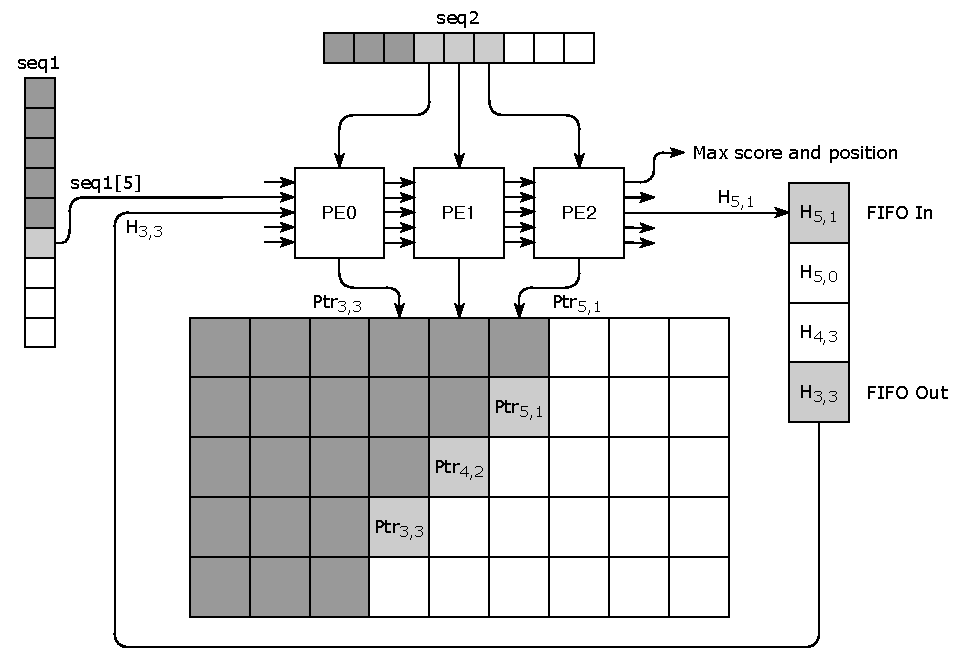
\includegraphics[width=0.9\textwidth]{figs/med_systolic_array.pdf}
    \caption{An overview of the systolic array}
    \label{fig:Medium_Systolic_Array}
\end{figure}

\begin{figure}
    \centering
    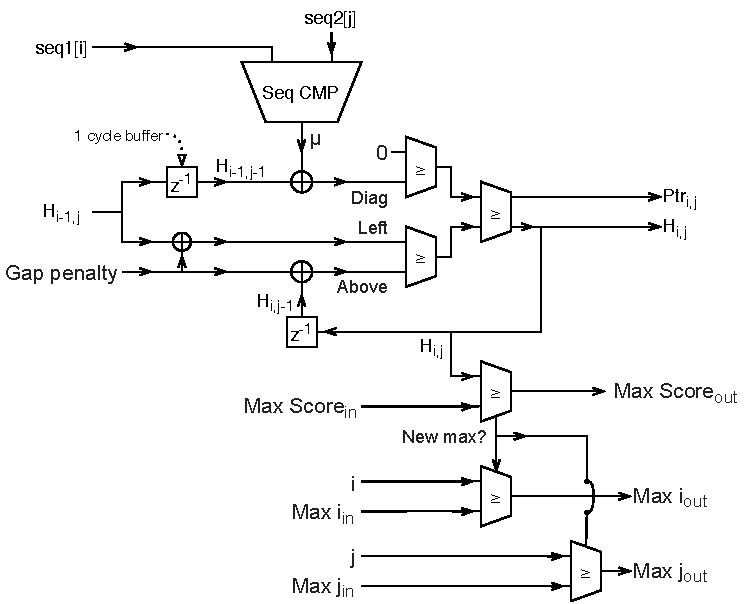
\includegraphics[width=0.75\textwidth]{figs/pe_cell.pdf}
    \caption{The structure of a single processing element in the systolic array}
    \label{fig:PE_Cell}
\end{figure}

\subsection{Device memory limitations}
\label{sec:Memory_in_SV}

The limiting factor is needing to store this array of pointers.
Each pointer can be one of four values, so $\SI{2}{\bits}$ per pointer was required.
For two sequences of lengths $N$ and $M$, $N\times M$ such pointers are required.
In each cycle each PE could be writing out a pointer, and this bandwidth requirement also influenced the choice of what type of memory to use.

There are several different types of memory on the development board I used, with different characteristics (\cref{tab:FPGA_Memories}).
Bandwidth limitations to the highest capacity memory devices (the $\SI{64}{\mebi\byte}$ SDRAM for the FPGA, and the $\SI{1}{\gibi\byte}$ SDRAM for the HPS) would have limited the size of the systolic array to $8$ or $32$ PEs respectively, due to their 16-bit and 64-bit buses.
I instead chose to use the M10K embedded memory blocks, which is the largest collection of memory that does not have these bandwidth limitations.

Instead, the design was limited by the number of M10K blocks available.
There are $397$ M10K blocks on the board I was using, giving $\SI{3970}{\kibi\bit}$ of total memory; approximately 2 million possible pointers or a $1425\times1425$ grid.
In practice, $5$ M10K blocks were used in the interface between the HPS and FPGA, and the FIFO needed to be stored.
The FIFO is either $N$ or $M$ $\SI{16}{\bit}$ twos-complement integers long.
On top of this, each processing element needs exclusive access to the memory blocks for each part of the grid, if each processing element is to write every cycle.
Sharing blocks between PEs would have added complexity, and likely caused delays and hazards in the design.

With these constraints in mind, I chose the maximum sequence lengths of this implementation to be $1024\times1536$ symbols.
This grid can fit in $384$ M10K blocks, using $96.7\%$ of the blocks available.
The FIFO is $1024$ words long, and fits in $2$ M10Ks.
The systolic array had $48$ PEs, with each PE writing to $8$ M10K blocks of pointer grid.
Due to the factor of $3$ in $1536$, the length of the systolic array needs to be a multiple of $3$ to allow each M10K to be assigned to exactly one PE.
Due to this addressing constraint, the next largest systolic array that would work under this arrangement would have $96$ elements each with $4$ M10Ks.
However, the $48$ PE array requires $62\%$ of the logic elements when aligning DNA, and $93\%$ when aligning proteins (\cref{sec:FPGA_utilisation}).
In both cases, doubling the number of PEs was not possible without a larger FPGA.

With a more modern FPGA, such as a similarly priced Cyclone 10 FPGA to the Cyclone V when that was first sold, would have nearly double the logic elements and quadruple the amount of embedded memory \cite{Cyclone10}.
My design would likely be able to be instantiated as a $96$ PE array, and could align sequences of lengths $2048$ and $3072$, probably at a higher clock speed as well.

\subsection{Back-tracing}
\label{sec:Back_tracing_in_SV}

Back-tracing involves starting at the best cell found by the systolic array, and following the pointers through the grid.
A minor challenge was that it takes a cycle between requesting an address from a M10K block and getting the data out.
It is possible to pipeline requests, where the next address is requested whilst the previous address is being read out, but this would have been complex to implement.
This meant that back-tracing takes two cycles per aligned symbol, with an upper bound on the number of cycles spent back-tracing being $2\times(N+M)$.

I chose not to pipeline this because back-tracing only takes a small amount of the overall execution time.
When aligning sequences of lengths of $1024$ and $1536$, only $13\%$ of the time is spent back-tracing (\cref{sec:Processing_time_on_FPGA}).
Using Amdahl’s law, if I could improve back-tracing to only take one cycle per symbol, the expected speedup is $1.07$ times; it would not have a significant impact overall processing time.
$$Speedup = \frac{1}{87\% + \frac{1}{2}\times 13\%} = 1.07 $$

\subsection{Processing time}
\label{sec:Processing_time_on_FPGA}
It is possible to derive exactly the amount of time it will take to align two sequences when working with FPGAs with constant clock frequencies.
For the design described above, with $48$ PEs in the systolic array, and sequences of lengths $N$ and $M$, the runtime is as follows.

For a 48-column section of the grid, it takes $48$ cycles for the last column to begin being evaluated, and then $N$ cycles to reach the bottom of that last column, requiring $N+48$ cycles in all.
One additional cycle is required, to find the diagonal score for the first column.
In conclusion, each 48-column section of the grid takes $N+49$ cycles to evaluate.

The number of 48-column segments in the grid is $\left \lceil \frac{M}{48} \right \rceil$.
Even when processing the last segment, which may have fewer than $48$ columns to consider, the device must wait $N+49$ cycles because the best score and location needs to propagate to the last PE, from which it is read by the back-tracing logic.
Combining this, the number of cycles required to produce the grid is ${(N+49) \times \left \lceil \frac{M}{48} \right \rceil}$

As discussed in the \cref{sec:Back_tracing_in_SV}, the amount of time required by the back-tracing logic is bounded by $2\times(N+M)$, so the number of cycles required for an alignment is:
$$\text{Runtime} = (N+49) \times \left \lceil \frac{M}{48} \right \rceil + 2 \times (N+M)$$

This expression is $O(NM)$.
Evaluating this expression with the maximum sequence lengths of $1024$ and $1536$ from previous section:
$$\text{Runtime} = (1024+49) \times \left \lceil \frac{1536}{48} \right \rceil + 2 \times (1024+1536) = \SI{39456}{\cycles}$$
Where $5120$ of the $\SI{39456}{}$ cycles ($13\%$) are spent back-tracing and the rest on filling the grid.
For the design which aligned DNA sequences I was able to clock my logic at $\SI{79}{\mega\hertz}$ using a PLL, so this pair of DNA sequences requires $\SI{499.4}{\micro\s}$ to execute.
Due to the additional complexity when aligning proteins my design could only run at $\SI{60}{\mega\hertz}$, so this pair of protein sequences requires $\SI{657.6}{\micro\s}$ to execute.
These limitations are discussed in \cref{sec:SV_Fmax}.

\subsection{Sequence similarity functions and scoring gaps}
\label{sec:Scoring_in_SV_impl}

Sequence similarity functions and gap penalty values were compiled into the hardware.
This reduces the flexibility of a compiled design, but this was sufficient for the testing I was doing.
For aligning nucleotides, I used a constant sequence similarity function and for aligning proteins I used the BLOSUM50 scoring matrix.
Representing one of four nucleotides takes $\SI{2}{\bits}$ but representing one of $22$ amino acids takes $\SI{5}{\bits}$.
This increased representational cost, alongside the quadratically scaled lookup table to align symbols, leads to the increased logic utilisation for the protein aligning circuit and also a lower maximum clock speed of that design (\cref{sec:FPGA_utilisation}).

I did not have the time to implement an affine gap scoring mechanism (\cref{sec:SW_gaps}) in my FPGA implementation, but the entire FPGA implementation was a project extension.
I expect it would not have had a major performance penalty.
The number of scores that need to be stored will triple (to cover three grids instead of one), but the systolic array only stores a small number of these scores to begin with.
The number of comparisons inside PEs would increase by two per cycle (one for each gap matrix), and only increase the comparison tree depth by one level.

\section{Repository overview}
\label{sec:Repo_overview}

My source code repository is divided into three sections (\lstinline{cpu_code}, \lstinline{gpu_code}, \lstinline{fpga_code}) which reflect the three major implementations of my project.
All code in it has been written from scratch, apart from the FPGA-HPS interfaces (\lstinline{fpga_code/systemverilog/*_avalon.sv}, and the contents of \lstinline{fpga_code/c_interface/}) which are based on code from my supervisor Peter Rugg, as discussed in \cref{sec:Starting_Point}.
A detailed overview can be found in \cref{fig:Repo_tree}.

% !TeX root = ./diss.tex

\DTsetlength{0.2em}{1em}{0.2em}{1pt}{4pt}
\begin{figure}[H]
\dirtree{%
    .1 /.
    .2 cpu\_code\DTcomment{C implementation}.
        .3 correctness\_tester.c \DTcomment{Basis for correctness testing across implementations}.
        .3 helpers.c \DTcomment{Utility functions}.
        .3 main.c \DTcomment{Entry point; rudimentary command line interface}.
        .3 nw.c \DTcomment{Initial global alignment implementation}.
        .3 sw.c \DTcomment{Local alignment implementation, quadratic and linear space}.
        .3 swParallel.c \DTcomment{Multi-threaded local alignment implementation}.
        .3 swGotoh.c \DTcomment{Affine gap implementation, quadratic and linear space}.
        .3 swGotohParallel.c \DTcomment{Multi-threaded affine gap alignment implementation}.
    .2 gpu\_code\DTcomment{CUDA implementation}.
        .3 helpers.cu \DTcomment{Utility functions}.
        .3 main.cu \DTcomment{Entry point; rudimentary command line interface}.
        .3 sw.cu  \DTcomment{Local alignment implementation, quadratic and linear space}.
        .3 swSingleBlock.cu \DTcomment{Quadratic space local alignment, without block-parallelism}.
        .3 swGotoh.cu \DTcomment{Affine gap implementation}.
    .2 fpga\_code\DTcomment{FPGA implementation}.
        .3 c\_interface \DTcomment{C Interface for ARM HPS}.
            .4 sequence\_reader.c \DTcomment{Reading sequences from files}.
            .4 start.c \DTcomment{Interface with FPGA}.
        .3 systemverilog \DTcomment{SystemVerilog implementation}.
            .4 datatypesPkg.sv \DTcomment{Types of signals used}.
            .4 macro.vh \DTcomment{Implementation-wide macros to change types of sequences}.
            .4 pe\_bram.v \DTcomment{BRAM for grid of pointers}.
            .4 fifo\_16b\_1024w.v \DTcomment{BRAM FIFO for storing previous column of scores}.
            .4 backtrace.sv \DTcomment{Backtracing through a grid of registers}.
            .4 backtrace\_with\_ram.sv \DTcomment{Backtracing through a grid in M10K BRAM}.
            .4 pe.sv \DTcomment{Single processing element where pointer grid is registers}.
            .4 pe\_with\_ram.sv \DTcomment{Single processing element where pointer grid is BRAM}.
            .4 short\_solver.sv \DTcomment{Systolic array for sequences the length of the array}.
            .4 short\_solver\_avalon.sv \DTcomment{Avalon FPGA-HPS interface for \lstinline{short_solver}}.
            .4 med\_solver.sv \DTcomment{Systolic array for sequences of lengths $1024 \times 1536$}.
            .4 med\_solver\_with\_ram.sv \DTcomment{\lstinline{med_solver} but using BRAM for pointer grid}.
            .4 med\_solver\_with\_ram\_avalon.sv \DTcomment{Main Avalon FPGA-HPS interface}.
            .4 tb\_blosum.sv \DTcomment{Various testbenches (\lstinline{tb_*})}.
            .4 tb\_med\_solver.sv .
            .4 tb\_med\_solver\_with\_ram.sv .
            .4 tb\_pe.sv .
            .4 tb\_short\_seq.sv .
            .4 tb\_short\_solver.sv .
        .3 quartus \DTcomment{Configuration files from my Quartus Lite project}.
}
\caption{Header files (of extensions \lstinline{.h} and \lstinline{.cuh}) have been omitted from for brevity, and always correspond to a code file. Makefiles have also been omitted.}
\label{fig:Repo_tree}
\end{figure}



% !TeX root = ../diss.tex

\chapter{Evaluation}
I performed two investigations to evaluate my work; to find out whether my implementations were correct, and their performance characteristics.

\section{Correctness testing}
\label{sec:Correctness_eval}

I tested whether my designs would correctly align sequences as I produced them.
After developing each implementation, I thoroughly tested it to ensure that it would produce a correct and optimal alignment for any pair of sequences.
I did this to stop errors from being carried over from one implementation to the next, as outlined in \cref{sec:Methodology_prep}.

Each implementation needs to produce alignments that are correct and optimal.
A correct alignment will produce two strings which are substrings of the input sequences, after gap symbols (\lstinline{-}) are removed from the alignment sequences.
An optimal alignment will have the highest score of any of the possible alignments between the sequences.
There can be multiple optimal alignments, with the same score, when the \lstinline{max} functions in the implementations choose different pointers when the argument of the \lstinline{max} functions have the same value (\cref{sec:SW_DP}).

I used the alignment program in EMBOSS \cite{EMBOSS} to test my C implementation, and then used my C implementation to test my CUDA and SystemVerilog implementations.
I used EMBOSS to find the scores of optimal alignments between sequences and checked my program produced an alignment with the same score.
My C implementation would also check if alignments were valid, and this code was checked against the substring checker built into Python.

To test the CUDA and SystemVerilog implementations, the C program was used to check the scores of the alignments, and to check that the alignments were valid.
A small set of test sequences was also used during the development process, especially when simulating the SystemVerilog, but each implementation was tested thoroughly when I finished working on it.

This was the testing approach applied to a large set of test sequences. Many of the sequences were randomly generated from lengths $1$ to $\SI{131072}{}$, and others were specific edge cases (such as identical sequence pairs, or pairs with no shared characters).
I also used the set of proteins that relate to humans or mice in SwissProt database \cite{UniProt}; a total of $\SI{37393}{}$ sequences ranging in length from $2$ to $\SI{35213}{}$ symbols. Approximately $\SI{100000}{}$ pairs of sequences were tested for each implementation.

No issues were found in the last correctness testing run for each of my implementations, thus I believe all three correctly and optimally align sequences.

\section{Performance testing}
\label{sec:Performance_eval}

\subsection{Testing approach}
\label{sec:Performance_approach}

I also tested the performance of my different implementations, mainly by measuring the amount of time they took to align sequences, comparing the implementations and different variants of the same implementation.
DNA and protein sequence datasets based on real-world data were not ideal for testing sequence alignment programs.
DNA datasets tend to be made up of very long sequences (often significant fractions of a chromosome, which are made up of hundreds of thousands if not millions of symbols), and the protein dataset SwissProt \cite{UniProt} did not have sequences of the lengths I wanted to test against.

Instead, I produced a synthetic dataset to evaluate my program.
I resampled the distribution of amino acids in proteins in humans \cite{AminoAcidFreqs} to produce protein sequences, and I resampled the distribution of codons (trigrams of nucleotides) \cite{CodonFreqs} to produce DNA sequences.
This meant they were similar to true sequences, and because they were randomly generated pairings were unlikely to form edge cases in alignments.

\subsubsection{Testing environment}
\label{sec:Testing_environment}
All tests were run on my Dell XPS 15 9570 laptop, running Ubuntu 18.04 LTS.
It has an Intel i7-8750H CPU, an Nvidia GTX 1050 Ti GPU, and 16 GB of DDR4 RAM.

Each performance test was run $10$ times, and the averages are plotted in the figures, with error bars of $\pm\sigma$.
For several figures, this interval is very small and the error bars are occluded by the point markers.
When sampling $10$ times, this $\pm\sigma$ error bar provides a $99.84\%$ confidence interval if the samples are normally distributed.
Trendlines are linear unless otherwise stated.

\subsection{Comparing implementations}
\label{sec:Comparing_implementations}

Comparisons between all three implementations are limited by the SystemVerilog implementation, which can only align sequence pairs shorter than $1024\times1536$.
\Cref{fig:All3} shows the throughput of each implementation (the average amount of time taken to align a pair of sequences), in milliseconds.
Using increased parallelism and specialisation, the FPGA is able to significantly outperform the CPU and GPU for shorter sequences.

For short sequences, not as many threads are required, so the better single-threaded performance of the CPU dominates over the GPU.
However, when evaluating against long sequences, the GPU implementation is able to use increased parallelism to outperform the CPU.
\Cref{fig:All3_Big} shows the throughput when aligning a sequence of length $\SI{32768}{}$ against the given length.

Also included on \cref{fig:All3_Big} is an extrapolated speed for the FPGA, using the formula derived in \cref{sec:Processing_time_on_FPGA}, with the result doubled.
The design I produced was space limited, but only the most expensive FPGAs have enough embedded memory to align these long sequences with the quadratic space algorithm.
Instead, a linear space approach is required, doubling the amount of arithmetic required, so \cref{fig:All3_Big} plots double the value given by the formula in \cref{sec:Processing_time_on_FPGA}.
This is only a rough estimate, an actual design is likely to have a different number of processing elements and clock speed to my quadratic space design.

Using this approximation, there is a small difference between the FPGA and GPU.
Although the FPGA design is highly specialised, the clock speed is much lower than the GPU and only allows for $48$ concurrent cell evaluations, whereas the GPU can execute $768$ threads simultaneously.
This comparison is not completely fair due to the age difference between the devices (\cref{sec:FPGA_prep}), and a newer and larger FPGA might be able to perform significantly better than the GPU.

\begin{figure}[H]
    \centering
    \begin{subfigure}{.49\textwidth}
      \centering
      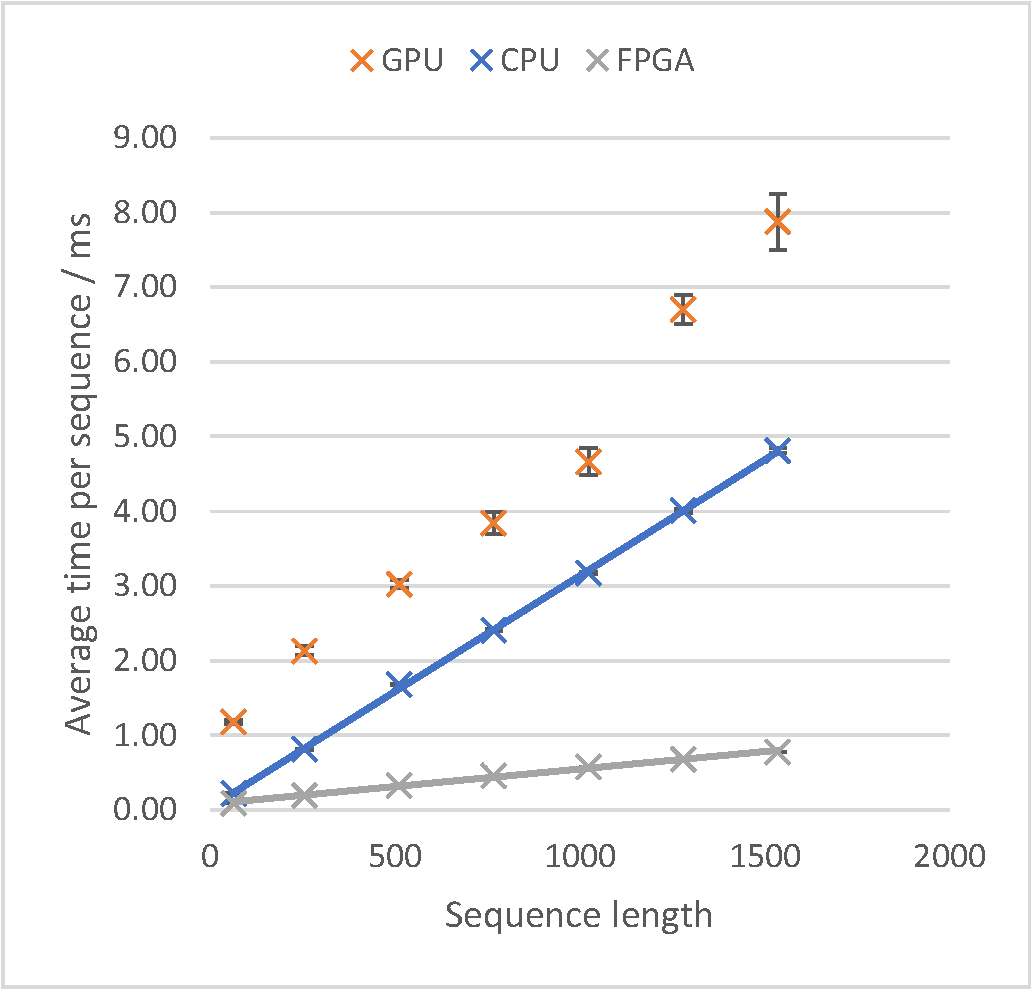
\includegraphics[width=\linewidth]{figs/eval/all3_blosum.pdf}
      \caption{Aligning two proteins using BLOSUM50 \mbox{substitution} matrix. CPU: $R^2=0.9997$, FPGA:~${R^2=0.9957}$}
      \label{fig:All3_BLOSUM}
    \end{subfigure}%
    \hfill
    \begin{subfigure}{.49\textwidth}
      \centering
      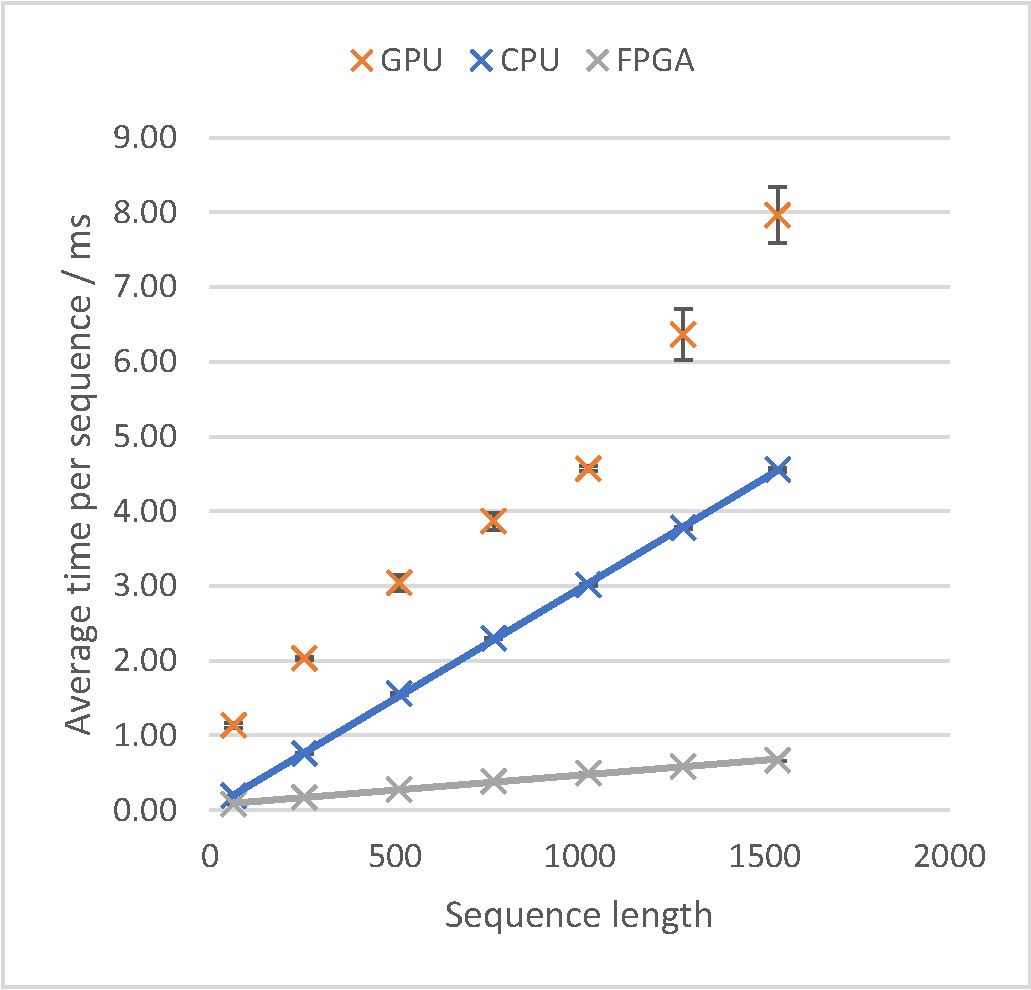
\includegraphics[width=\linewidth]{figs/eval/all3_dna.pdf}
      \caption{Aligning two DNA sequences using a constant similarity function. CPU: $R^2=0.9999$, FPGA:~${R^2=0.9967}$}
      \label{fig:All3_DNA}
    \end{subfigure}
    \caption{Throughput of aligning a sequence of length $1024$ against the given length}
    \label{fig:All3}
\end{figure}

\begin{figure}[H]
    \centering
    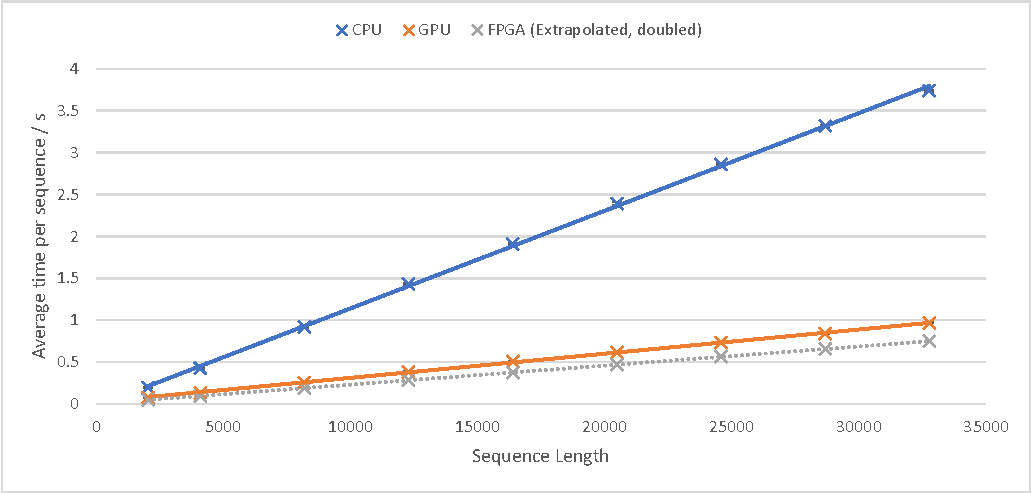
\includegraphics[width=\textwidth]{figs/eval/all3_big.pdf}
    \caption{Throughput of aligning two proteins of length $\SI{32768}{}$ against the given length, using BLOSUM. CPU: $R^2=0.9995$, GPU: ${R^2=0.9994}$}
    \label{fig:All3_Big}
\end{figure}

\subsection{C implementation}
\label{sec:C_eval}

\subsubsection{Setting implementation parameters}
\label{sec:C_params_eval}

The first tests were to set the implementation parameters, values that change how the program performs but do not change the output.
One parameter is the point at which the linear space program has sufficiently subdivided the alignment and calls the quadratic space program instead.
To set this crossover point, a set of $12$ alignments of two $\SI{32768}{}$-symbol long sequences of proteins were performed by the parallel linear space implementation, with the crossover length set at different points.
The impact of this (which can be seen in \cref{fig:C_Crossover}) was minor, but smaller crossover points appeared to be slightly better so I used a crossover value of $1024$ symbols.
Setting the value below $1024$ led to instability due to the number of threads required.

\begin{figure}[H]
    \centering
    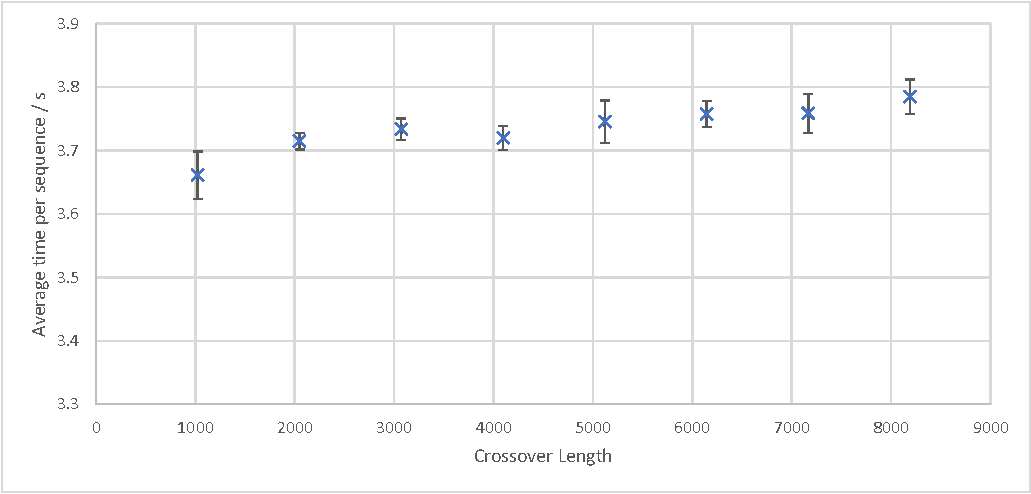
\includegraphics[width=\textwidth]{figs/eval/c_crossover.pdf}
    \caption{Throughput of aligning two proteins both of length $\SI{32768}{}$, using BLOSUM, at different crossover points. Note the y-axis starts at $\SI{3.3}{\s}$.}
    \label{fig:C_Crossover}
\end{figure}

The other parameter to consider was the number of threads that could be working at one time, which was controlled using a semaphore (\cref{sec:Multi_threaded_C_impl}).
This was tested by measuring the time it took to align $24$ pairs of proteins of lengths $\SI{32768}{}$, and turned out to be a demonstration of simultaneous multithreading, and the results are shown in \cref{fig:C_Cores}.

There were no significant speedups when allowing more than $6$ threads to work, but this did very gradually speed up till $12$ threads.
However, the amount of time spent by threads resident in the CPU (user time) increased nearly linearly until $12$ threads.
Up to $12$ threads can be resident in a 6-core CPU with Intel's Hyperthreading technology (thus the linear increase in user time) but there are only enough resources in a core for an average of one thread's work to be done (thus the minor changes in wall time).
The minor decrease in wall time between $6$ and $12$ threads (between $\SI{4.13}{\s}$ and $\SI{3.56}{\s}$ respectively) is probably due to the two threads occasionally being able to share resources on the CPU, extracting a $16\%$ speedup.
Based on this information, I chose to run my tests with up to $12$ threads working at one time.

\begin{figure}
    \centering
    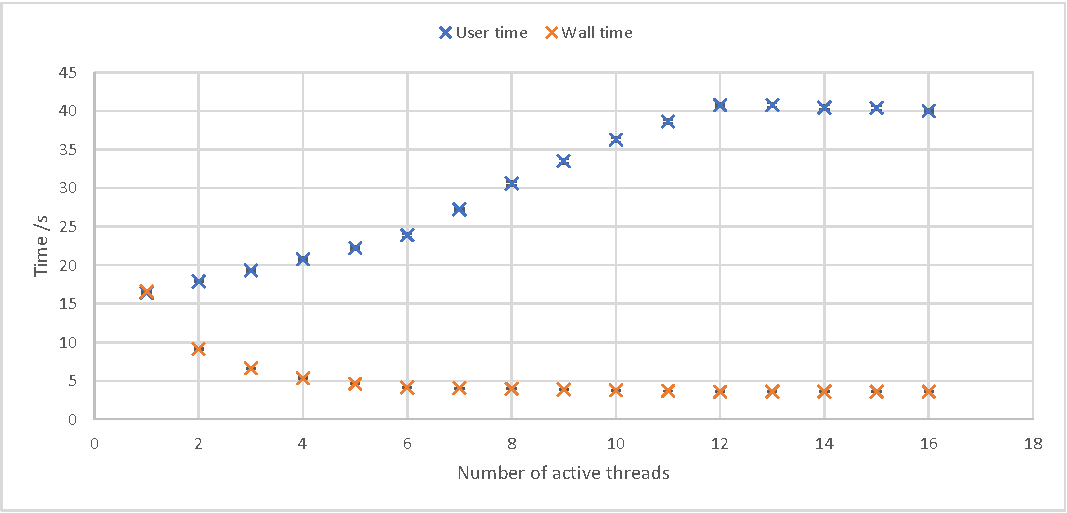
\includegraphics[width=\textwidth]{figs/eval/c_cores.pdf}
    \caption{Time taken to aligning $24$ pairs of proteins both of length $\SI{32768}{}$, using BLOSUM, using different numbers of cores}
    \label{fig:C_Cores}
\end{figure}

\subsubsection{Quadratic, Linear Space, and Multithreaded implementations}
\label{sec:C_impls_eval}

Two metrics to compare the different implementations in C are latency and throughput.
Throughput measures the average time spent on each sequence, whereas latency measures the time between starting and finishing an alignment.
\Cref{fig:C_Space_IL} shows the throughput of the different implementations, measured by allowing up to $12$ threads to work on a set of alignments.
The linear space algorithms will use the quadratic space algorithm to align sub-sequences shorter than $1024$ symbols, though significant differences are not seen until aligning sequences of lengths $\SI{16384}{}$ and $\SI{32768}{}$ symbols.
One reason for this divergence is decreasing parallelism for the quadratic space algorithm as the space requirements grew, because fewer alignments could happen at the same time due to lack of memory.

In \cref{fig:C_Space_IL} the linear parallel implementation can use more than one thread to perform an alignment, whereas the simple linear version only uses one thread per alignment.
The number of threads used by an alignment does not affect throughput because the total amount of work done by the processor is the same, even if it can be distributed differently.
However, there is an impact on latency as shown in \cref{fig:C_Space_Ser}.

Latency was measured by sequentially aligning a set of sequences, as opposed to multiple sequences being aligned at a time when measuring throughput.
This is shown in \cref{fig:C_Space_Ser} and the parallelised implementation performs the best, because it recruits more than one CPU core.
The linear space variant involves double the arithmetic of the quadratic variant (\cref{sec:SW_Linear_Complexity}) yet only takes approximately $1.38$ times more time, likely due to less memory contention.
The parallel version was $2.41$ times faster than the linear space algorithm, compared to a maximum of $3$ times faster that could be expected (\cref{sec:Multi_threaded_C_impl}).

\begin{figure}
    \centering
    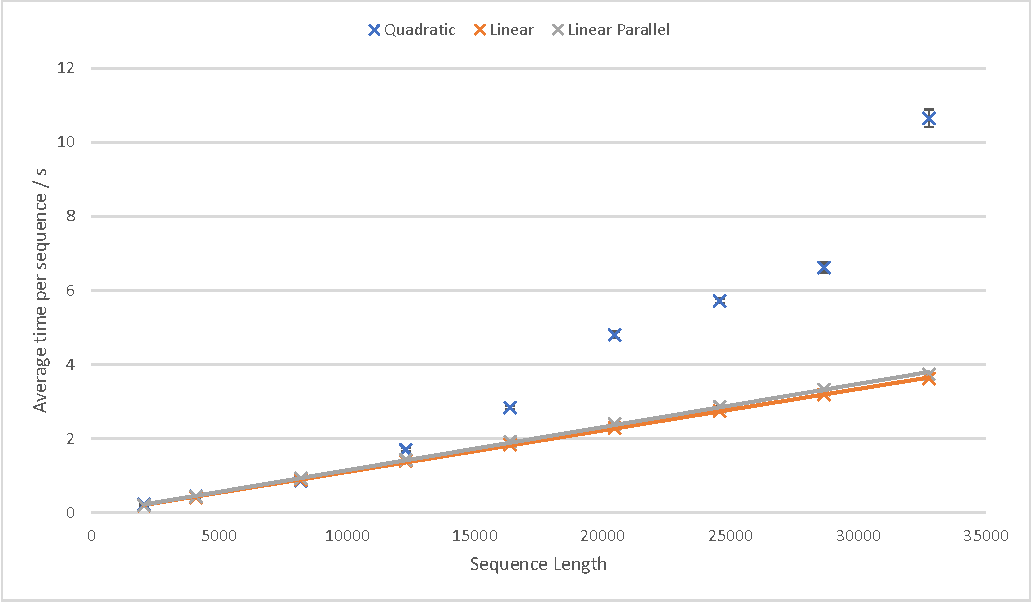
\includegraphics[width=\textwidth]{figs/eval/c_spaces_il.pdf}
    \caption{Throughput of aligning two proteins of length $\SI{32768}{}$ against the given length, using BLOSUM, using different C implementations. Linear: $R^2=0.9997$, linear parallel:~${R^2=0.9995}$}
    \label{fig:C_Space_IL}
\end{figure}

\begin{figure}
    \centering
    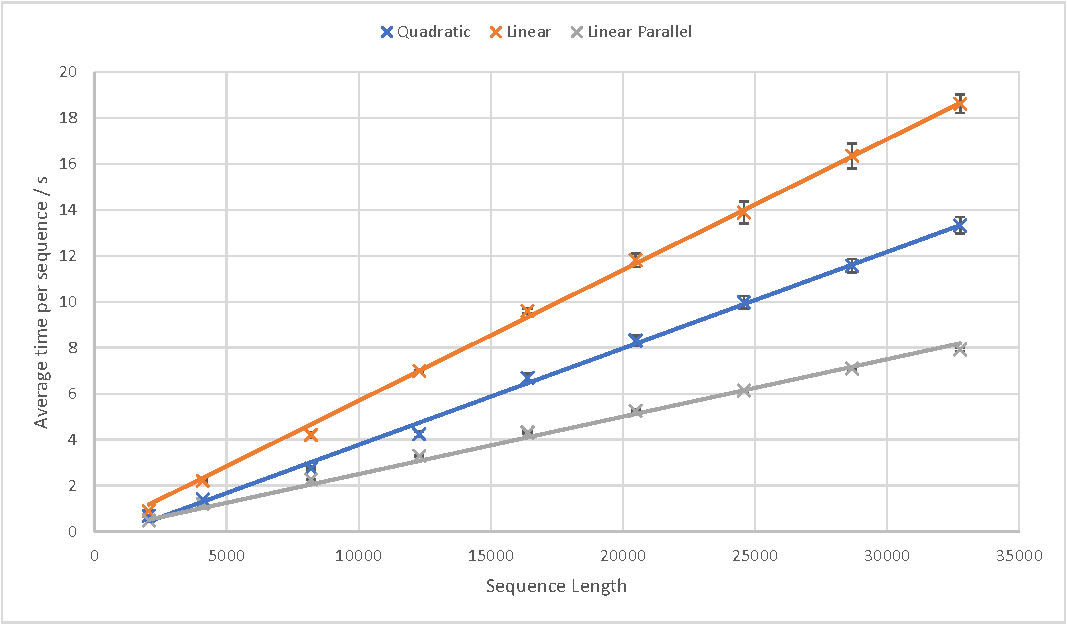
\includegraphics[width=\textwidth]{figs/eval/c_spaces_ser.pdf}
    \caption{Latency of aligning two proteins of length $\SI{32768}{}$ against the given length, using BLOSUM, using different C implementations. Quadratic: $R^2=0.9987$, linear: $R^2=0.9972$, linear parallel:~${R^2=0.9950}$}
    \label{fig:C_Space_Ser}
\end{figure}

\subsubsection{Sequence similarity functions and scoring gaps}
\label{sec:C_scoring_eval}

The impact of different methods of scoring methods (\cref{sec:SW_similarity_functions}) was also investigated; shown in \cref{fig:C_similarity_fun}.
I expected the gap between a constant function for proteins and BLOSUM, due to the cost of looking up values in the BLOSUM matrix.
I did not expect to see a gap between DNA and Protein constant functions, but this was likely due to differences in lengths of alignment for the different sets of sequences.
Interestingly, different results are found on the GPU (\cref{sec:CUDA_scoring_eval}).

The impact of different gap scoring methods (\cref{sec:SW_gaps}) was investigated; shown in \cref{fig:C_Gotoh}.
The extra arithmetic and memory required for affine gaps causes a $1.73$ time slowdown.

\begin{figure}
    \centering
    \begin{subfigure}{.49\textwidth}
      \centering
      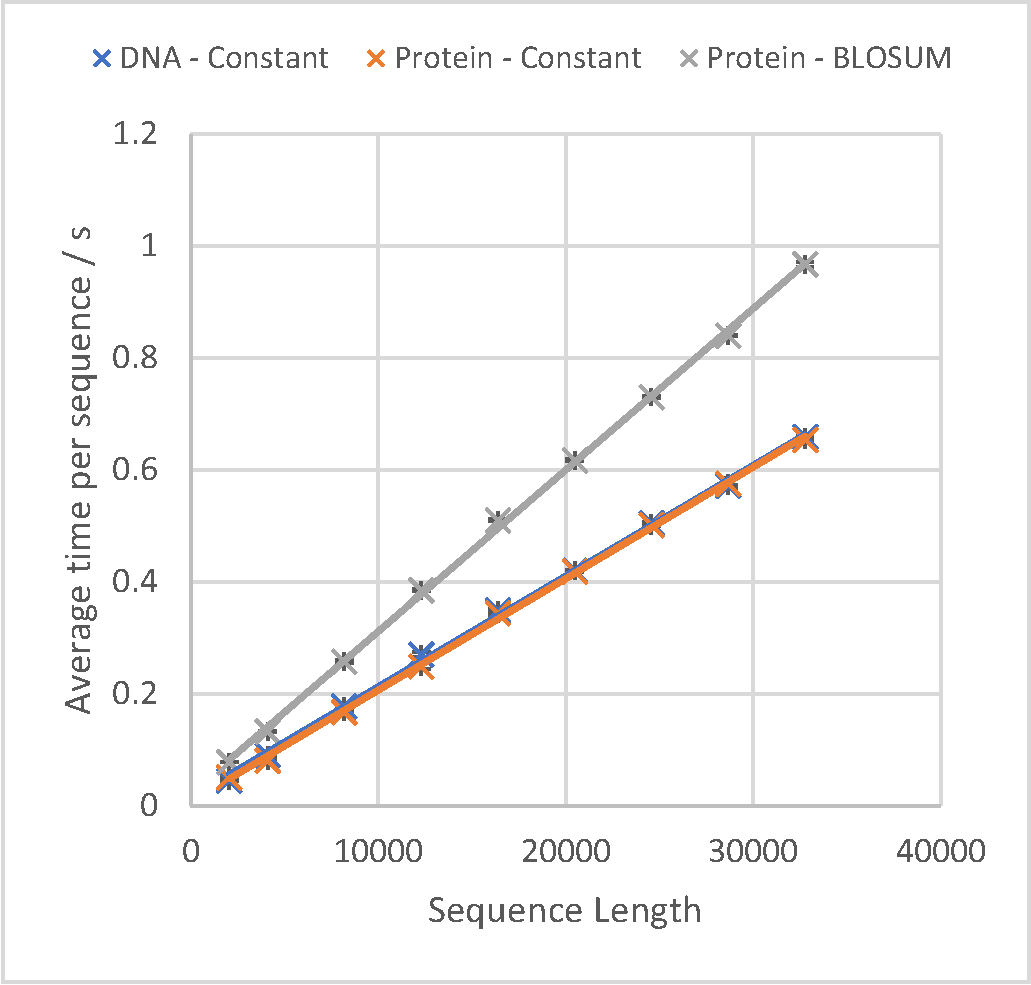
\includegraphics[width=\linewidth]{figs/eval/cu_similarity_f.pdf}
      \caption{Latency, using different similarity functions. DNA: $R^2=0.9998$, Constant~protein:~${R^2=0.9996}$, BLOSUM:~${R^2=0.9996}$}
      \label{fig:C_similarity_fun}
    \end{subfigure}
    \hfill
    \begin{subfigure}{.49\textwidth}
      \centering
      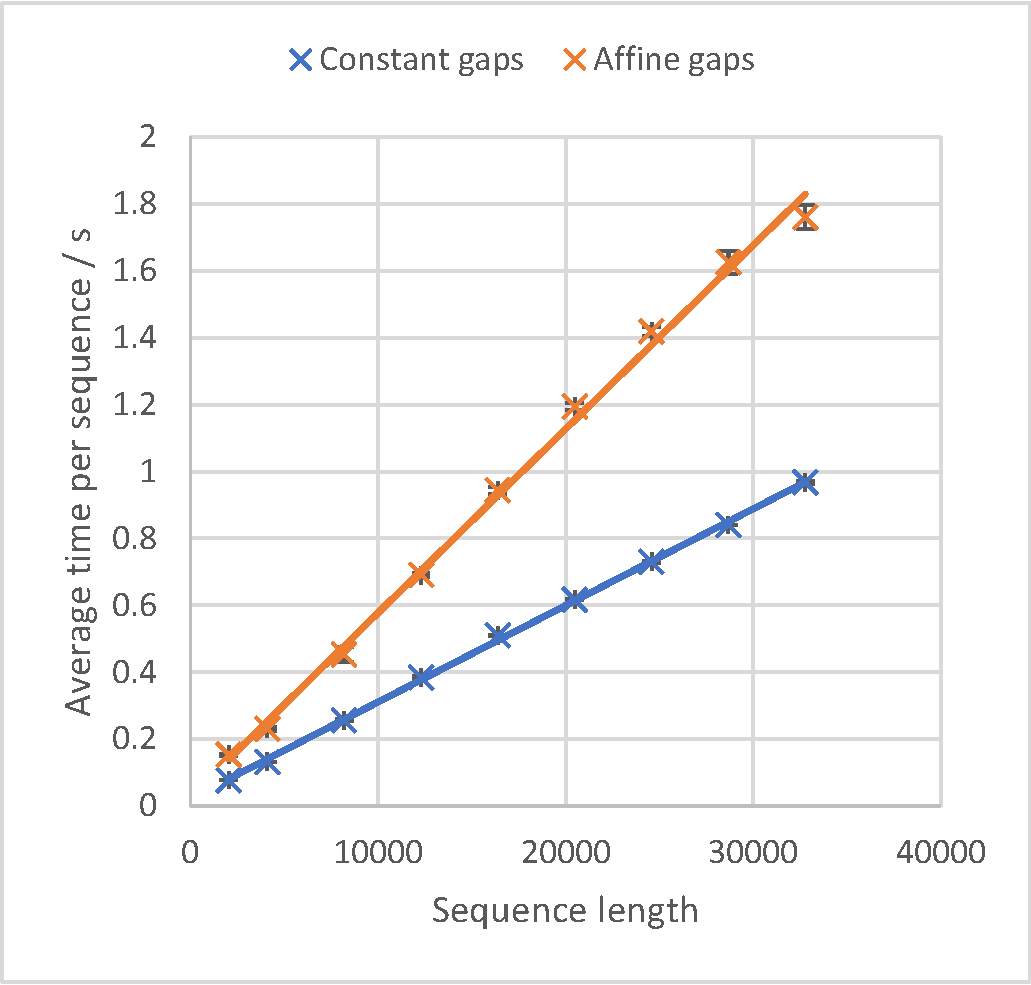
\includegraphics[width=\linewidth]{figs/eval/cu_gotoh.pdf}
      \caption{Latency using BLOSUM, using either constant or affine gaps. Constant: $R^2=0.9995$, \mbox{affine}~${R^2=0.9967}$}
      \label{fig:C_Gotoh}
    \end{subfigure}
    \caption{Latency of aligning two sequences of length $\SI{32768}{}$ against the given length, using different scoring mechanisms}
    \label{fig:C_Scoring}
\end{figure}

\subsubsection{Function occupancy}
\label{sec:C_occupancy}

I used Gprof to profile my C implementation and finding where time was spent during execution.
Gprof works by stopping the program every $\SI{0.01}{\s}$ and recording which function is being run at that time, to estimate the proportion of time spent in each function, $t$.
I profiled the alignment of a pair of sequences of lengths $\SI{32768}{}$ symbols and repeated this $10$ times.
The average function occupancy for quadratic space implementation can be found in \cref{tab:C_Quadratic_Occupancy}.

Memory access latency for the dynamic programming grid is counted in \lstinline{sw}, and for the sequence similarity matrix in \lstinline{matchBlosum}, and \lstinline{decideCell} is purely arithmetic, so there is a relatively even split between delays for arithmetic and for memory transactions.
The time taken for back-tracing was immeasurably small compared to the rest of the program.

\begin{table}
    \centering
    \begin{tabular}{|p{0.16\textwidth}|p{0.52\textwidth}p{0.08\textwidth}p{0.12\textwidth}|} \hline
        Function name & Description & Mean $t$ & Std. dev. $t$ \\ \hline
        {\ttfamily sw} & The top-level function which aligns sequences in quadratic space. & $47.23\%$ & $\pm0.886\%$ \\ \hline
        {\ttfamily decideCell} & Chooses the maximum of four scores, also returning a direction for the pointer grid, called by {\ttfamily sw}. & $42.61\%$ & $\pm1.45\%$ \\ \hline
        {\ttfamily matchBlosum} & The sequence similarity function, called by {\ttfamily sw}. & $10.16\%$ & $\pm0.983\%$ \\ \hline
        {\ttfamily backtrace} & Back-tracing routine & $0.000\%$ & $\pm0.000\%$ \\ \hline
    \end{tabular}

    \caption{Average function occupancy for quadratic space implementation in C}
    \label{tab:C_Quadratic_Occupancy}
\end{table}

The Gprof results for multi-threaded, linear space implementation were measured in a similar way and are summarised in \cref{tab:C_Linear_Occupancy}.
The quadratic space implementation was only used for a very small fraction of the time, with most of the time spent in the linear space function, or the two helper functions called by the linear space function.

\begin{table}
    \centering
    \begin{tabular}{|p{0.16\textwidth}|p{0.52\textwidth}p{0.08\textwidth}p{0.12\textwidth}|} \hline
        Function name & Description & Mean $t$ & Std. dev. $t$ \\ \hline
        {\ttfamily swLinear} & The top-level function which produces the middle column of scores using linear space, to decide how to subdivide the problem. This proportion does not include time spent in functions it calls. & $23.85\%$ & $\pm3.98\%$ \\ \hline
        {\ttfamily decideCell} & Chooses the maximum of four scores, called by {\ttfamily swLinear}. & $58.14\%$ & $\pm3.54\%$ \\ \hline
        {\ttfamily matchBlosum} & The sequence similarity function, called by {\ttfamily swLinear}. & $17.24\%$ & $\pm1.25\%$ \\ \hline
        {\ttfamily sw} & Quadratic space alignment function, called by {\ttfamily swLinear}. & $0.772\%$ & $\pm0.181\%$\\ \hline
        {\ttfamily backtrace} & Back-tracing routine for the quadratic space function. & $0.000\%$ & $\pm0.000\%$ \\ \hline
    \end{tabular}

    \caption{Average function occupancy for linear space implementation in C}
    \label{tab:C_Linear_Occupancy}
\end{table}

\subsection{CUDA implementation}
\label{sec:CUDA_eval}

\subsubsection{Setting implementation parameters}
\label{sec:CUDA_params_eval}

Like the C implementation (\cref{sec:C_params_eval}), some tuning parameters needed to be set before the CUDA implementation could be evaluated.
The first of which was the crossover point between quadratic and linear space algorithms, as discussed in \cref{sec:C_params_eval}, and is explored in \cref{fig:CU_Crossover}.
The quadratic space implementation can utilise more streaming multiprocessors as the sequences get longer, leading to stepped decreases as crossover increases.
However, large quadratic alignments can fully utilise the GPU so the graph plateaus, and GPU memory usage increases as longer sequences are aligned using quadratic space, so I set the crossover at $5120$ symbols.

\begin{figure}
    \centering
    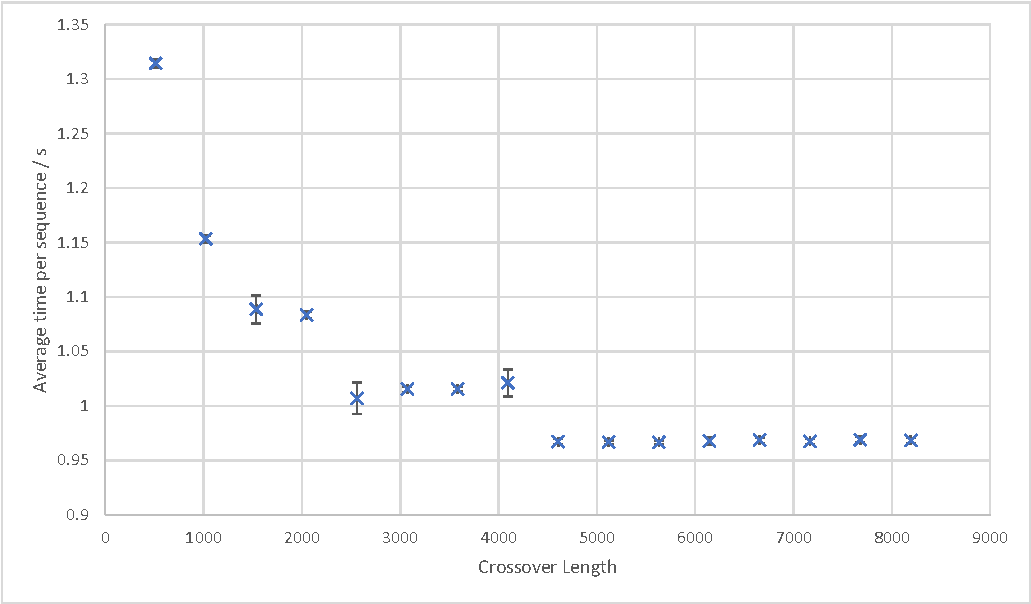
\includegraphics[width=\textwidth]{figs/eval/cu_crossover.pdf}
    \caption{Throughput of aligning two proteins both of length $\SI{32768}{}$, using BLOSUM, at different crossover points.}
    \label{fig:CU_Crossover}
\end{figure}

Also, the number of concurrent alignments needed to be decided, when measuring throughput.
To decide this, $24$ alignments were divided between different numbers of current threads, and the overall runtime is shown in \cref{fig:CU_Cores}.
The 12-thread version would not run due to the GPU running out of memory, and the figure shows that with $2$ or more threads there is a similar runtime, so two threads can produce enough work to fully utilise the GPU's resources.

\begin{figure}
    \centering
    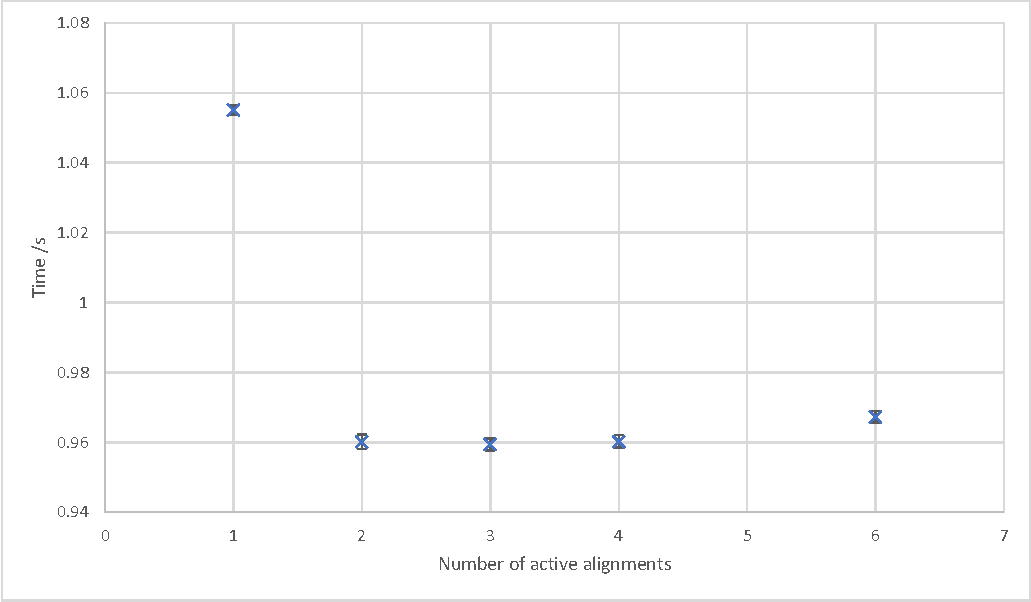
\includegraphics[width=\textwidth]{figs/eval/cu_cores.pdf}
    \caption{Time taken to aligning $24$ pairs of proteins both of length $\SI{32768}{}$, using BLOSUM, using different numbers of threads}
    \label{fig:CU_Cores}
\end{figure}

\subsubsection{Early and improved Quadratic Space implementations}
\label{sec:CUDA_single_multi_block_eval}

My initial quadratic space implementation only used one thread block, and I modified it to use more than one thread block to improve performance.
\cref{sec:Block_Parallelism_in_CUDA} contains the implementation details, and \cref{fig:CU_Multiblock} shows the difference in latency.

\begin{figure}
    \centering
    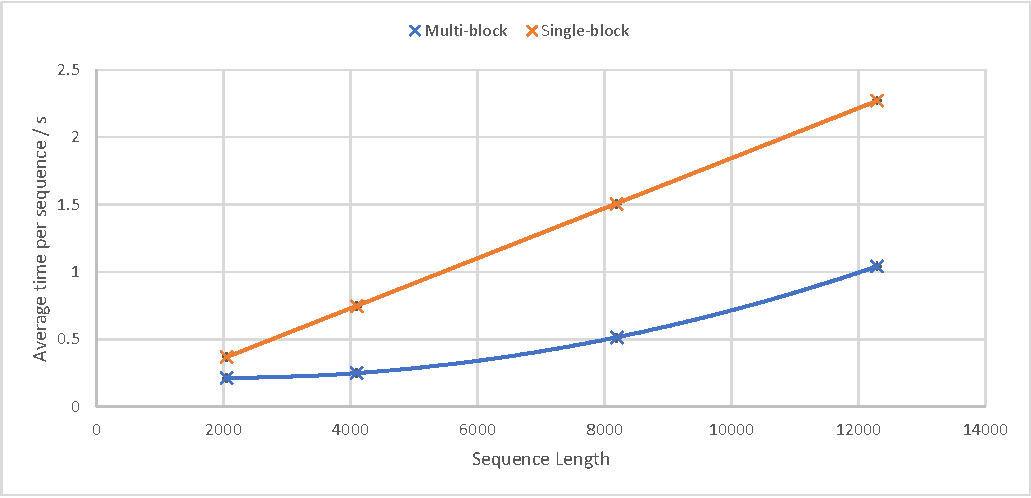
\includegraphics[width=\textwidth]{figs/eval/cu_single_block.pdf}
    \caption{Latency of aligning two proteins of length $\SI{32768}{}$ against the given length, using BLOSUM, the quadratic space algorithm. Multi-block trendline is quadratic, both $R^2=1.0000$}
    \label{fig:CU_Multiblock}
\end{figure}

\subsubsection{Quadratic and Linear Space implementations}
\label{sec:CUDA impls. eval}

Like the C implementation (\cref{sec:C_impls_eval}), latency and throughput are two helpful ways to compare the quadratic and linear space approaches.
\Cref{fig:CU_Spaces_Ser} shows the throughput of the different approaches, and the quadratic variant runs out of space after aligning sequences of lengths $\SI{32768}{}$ and $\SI{12288}{}$.
The decreasing throughput for longer sequences under the quadratic space variant is likely due to increased memory usage, so more time is spent on memory operations.
This is similar for latency (\cref{fig:CU_Spaces_Ser}).

There is a constant $\SI{86}{\milli\s}$ difference between throughput and latency for the linear space implementation, because the GPU cannot be fully utilised at the start and end of alignments, so these small amounts of idle time can be used by running two alignments at the same time.

\begin{figure}
    \centering
    \begin{subfigure}{.49\textwidth}
      \centering
      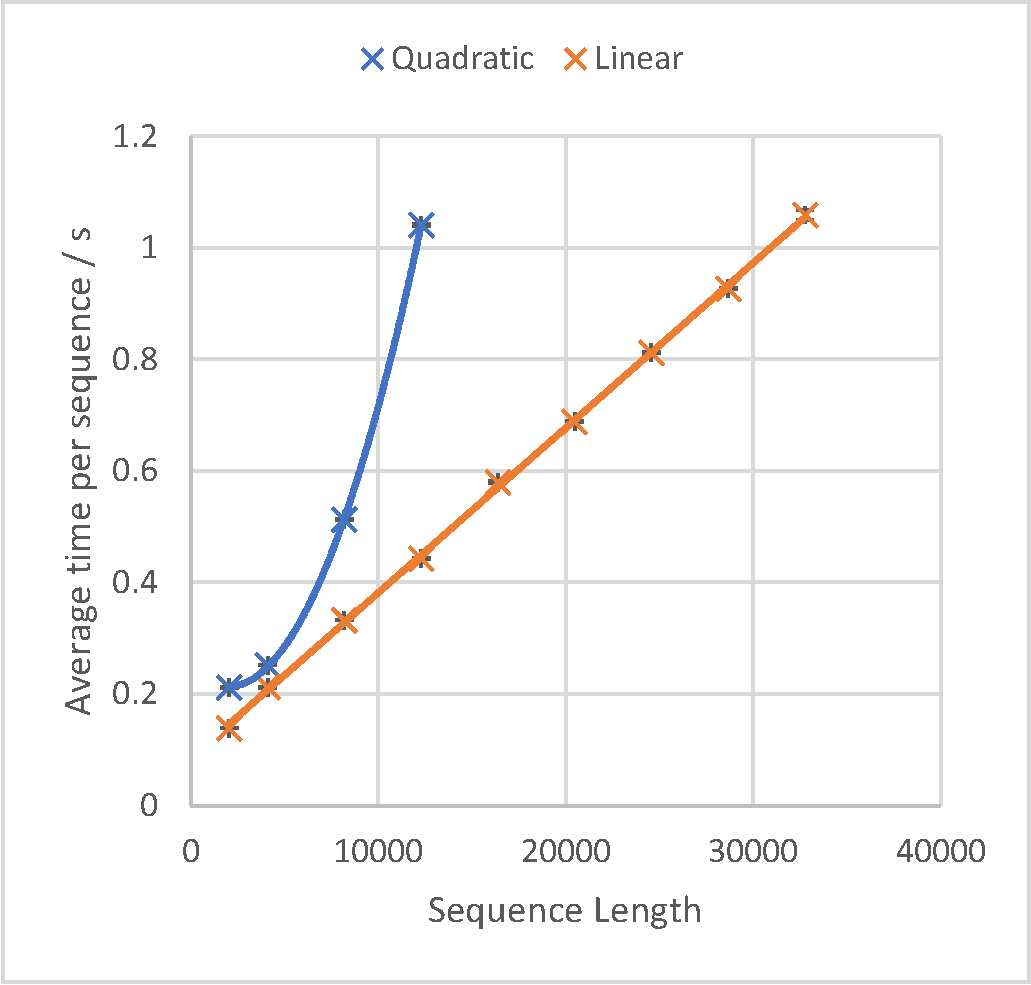
\includegraphics[width=\linewidth]{figs/eval/cu_spaces_ser.pdf}
      \caption{Latency. Quadratic: $R^2=1.000$, \mbox{Linear}:~${R^2=0.9996}$}
      \label{fig:CU_Spaces_Ser}
    \end{subfigure}
    \hfill
    \begin{subfigure}{.49\textwidth}
      \centering
      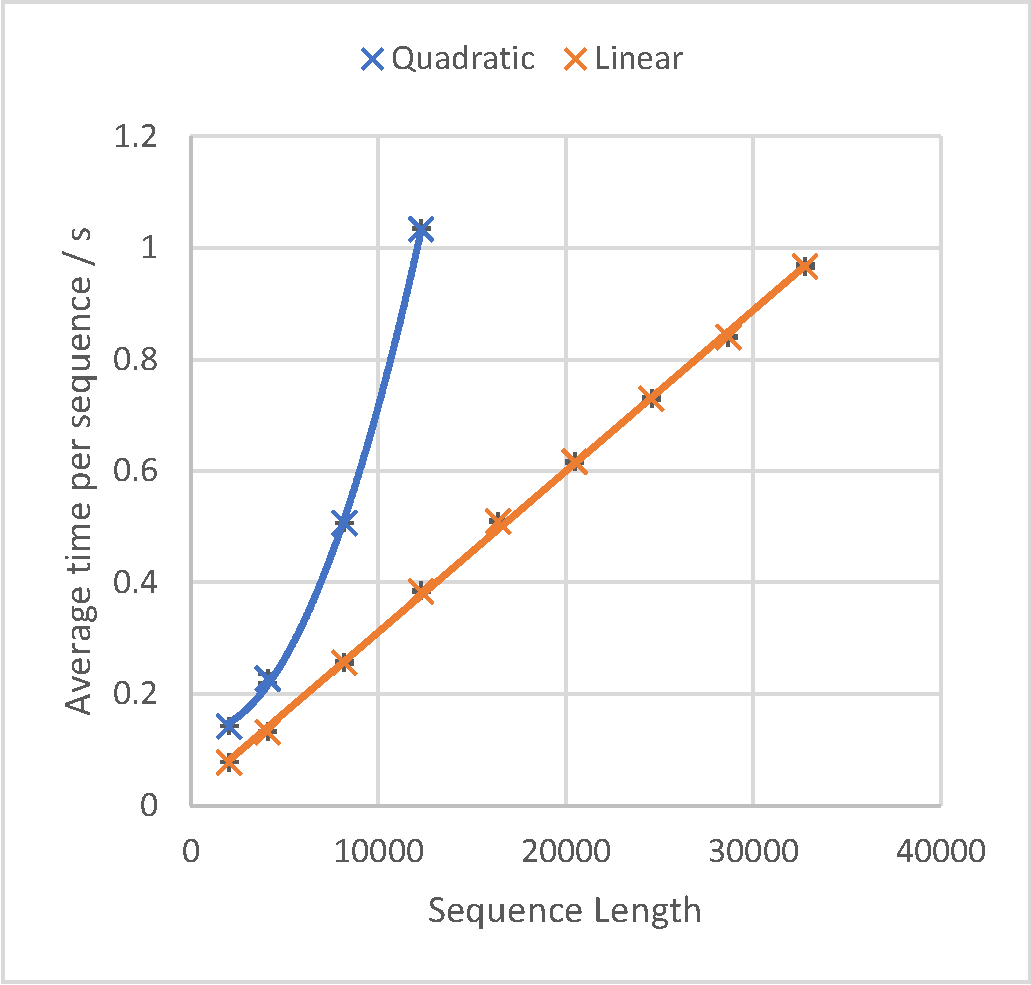
\includegraphics[width=\linewidth]{figs/eval/cu_spaces_il.pdf}
      \caption{Throughput. Quadratic: $R^2=0.9995$, \mbox{Linear}:~${R^2=0.9994}$}
      \label{fig:CU_Spaces_IL}
    \end{subfigure}
    \caption{Aligning two proteins of length $\SI{32768}{}$ against the given length, using BLOSUM, using different CUDA implementations. Quadratic has a quadratic trendline.}
    \label{fig:CU_Spaces}
\end{figure}

\subsubsection{Sequence similarity functions and scoring gaps}
\label{sec:CUDA_scoring_eval}

Similar to the C implementation, different scoring methods (\cref{sec:SW_Scoring}) were investigated.
The impact of using different sequence similarity functions is shown in \cref{fig:CU_similarity_fun}, with a significant difference between using a constant function and a lookup matrix like BLOSUM50.
There was no difference between the DNA and Protein constant functions, which unsurprising because the only thing that is different is the sequence alphabet.
However, there was a more pronounced difference in the C implementation (\cref{sec:C_scoring_eval}).

There was a significant performance penalty for using affine gaps rather than constant gaps, shown in \cref{fig:CU_Gotoh}, consistent with the additional arithmetic and memory required by affine gaps.

\begin{figure}
    \centering
    \begin{subfigure}{.49\textwidth}
      \centering
      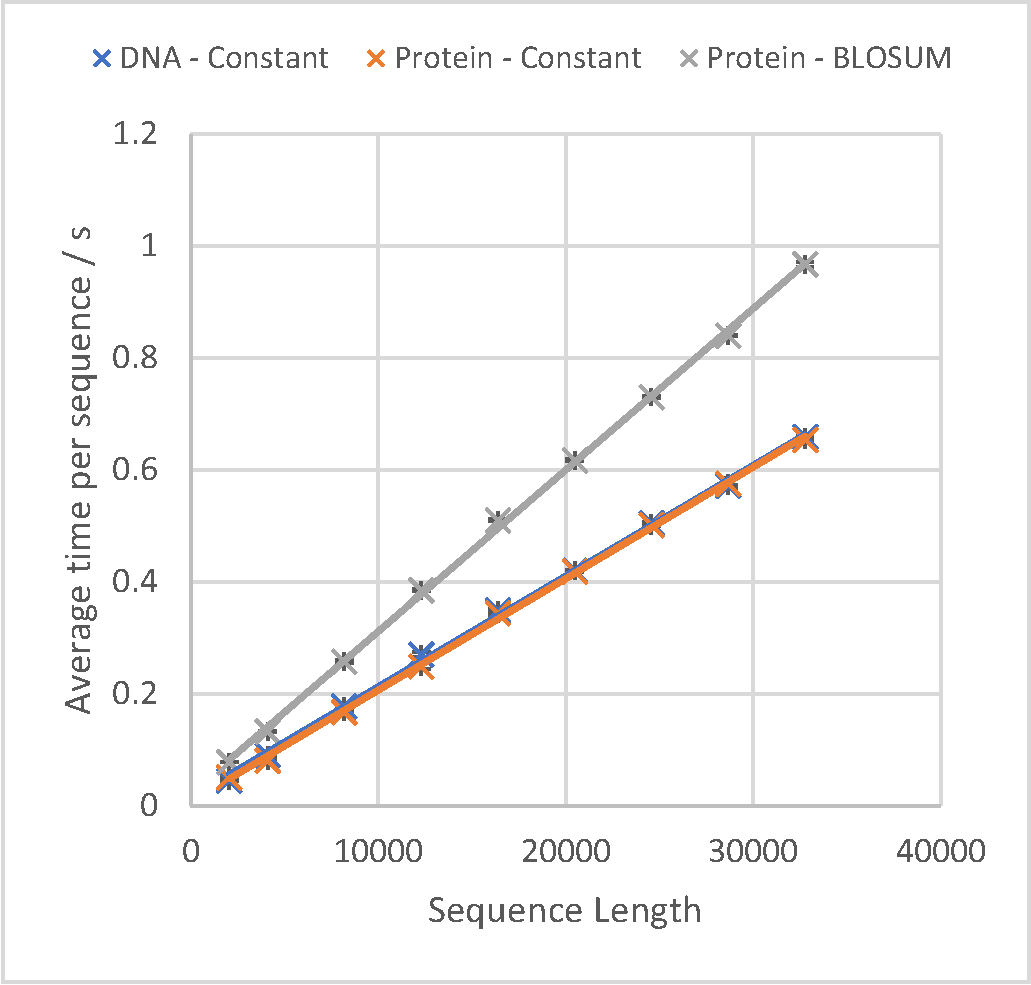
\includegraphics[width=\linewidth]{figs/eval/cu_similarity_f.pdf}
      \caption{Throughput, using different similarity functions. DNA: $R^2=0.9985$, Constant~protein:~${R^2=0.9993}$, BLOSUM:~${R^2=0.9994}$}
      \label{fig:CU_similarity_fun}
    \end{subfigure}
    \hfill
    \begin{subfigure}{.49\textwidth}
      \centering
      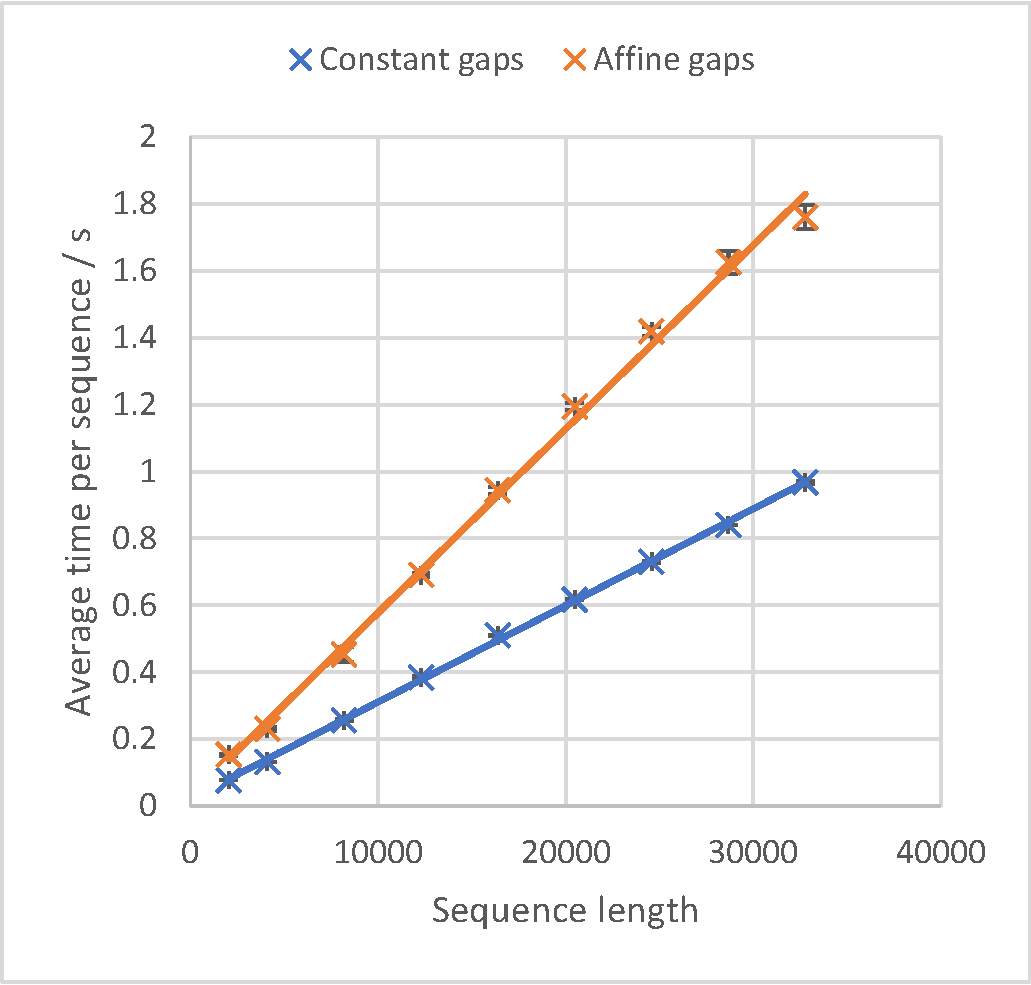
\includegraphics[width=\linewidth]{figs/eval/cu_gotoh.pdf}
      \caption{Throughput using BLOSUM, using either constant or affine gaps. Constant: $R^2=0.9994$, \mbox{affine}~${R^2=0.9964}$}
      \label{fig:CU_Gotoh}
    \end{subfigure}
    \caption{Throughput of aligning two sequences of length $\SI{32768}{}$ against the given length, using different scoring mechanisms}
    \label{fig:CU_Scoring}
\end{figure}

\subsubsection{Kernel occupancy}
\label{sec:CUDA_occupancy}
The time spent executing each kernel in a program can be measured using NVProf.
The results of using the quadratic space algorithm to produce $30$ alignments of lengths $\SI{12288}{}$ sequentially is shown in \cref{tab:CUDA_Quadratic_Occupancy}.
The alignment grid almost fills the whole GPU device memory.
The main kernel, \lstinline{sw_device}, is called multiple times for each alignment due to the way the problem is parallelised (\cref{sec:Block_Parallelism_in_CUDA}).
Back-tracing through the grid of pointers takes $5.41\%$ of execution time, whereas the C implementation spends an immeasurably small amount of time back-tracing (\cref{sec:C_occupancy}).
Moving the results from the GPU (the `device') to main memory is done by the back-tracing kernel, back-tracing is sequential so is slower on a GPU than a CPU, and filling the grid can be more effectively parallelised by the GPU.
Together this explains why back-tracing takes a larger proportion of time on the GPU than the CPU.

\begin{table}
    \centering
    \begin{tabular}{|p{0.18\textwidth}|p{0.09\textwidth}p{0.1\textwidth}p{0.105\textwidth}p{0.115\textwidth}p{0.08\textwidth}p{0.12\textwidth}|} \hline
        Name & Number of calls & Average time & Minimum time & Maximum time & Total time  & Total time prop. \\ \hline
        {\ttfamily sw} & $690$ & $\SI{12.1}{\milli\s}$ & $\SI{5.72}{\milli\s}$ & $\SI{31.1}{\milli\s}$ & $\SI{8.326}{\s}$ & $91.61\%$ \\
        {\ttfamily backtracer} & $30$ & $\SI{16.4}{\milli\s}$ & $\SI{16.3}{\milli\s}$ & $\SI{16.5}{\milli\s}$ & $\SI{491}{\milli\s}$ & $5.41\%$ \\
        CUDA {\ttfamily memcpy} Host to Device & $60$ & $\SI{4.50}{\milli\s}$ & $\SI{3.07}{\micro\s}$ & $\SI{9.33}{\milli\s}$ & $\SI{270}{\milli\s}$ & $2.97\%$ \\ \hline
    \end{tabular}

    \caption{Average function occupancy for quadratic space implementation in CUDA}
    \label{tab:CUDA_Quadratic_Occupancy}
\end{table}

The results of using the linear space algorithm to produce $30$ alignments of lengths $\SI{32768}{}$ sequentially are shown in \cref{tab:CUDA_Linear_Occupancy}.
This utilises the linear space improvements, for they are much larger than the crossover point of $5120$ (\cref{sec:CUDA_params_eval}), unlike aligning sequences of lengths $\SI{12288}{}$ as in \cref{tab:CUDA_Quadratic_Occupancy}.
My use of C++ templates results in two entries for each kernel evaluating grid cells, one for the alignments starting from the top-left ($1$), and the other when alignments can start from anywhere ($0$).
A similar proportion of time is spent back-tracing and \lstinline{addAndMaximise} is adds the two middle columns together and finds the maximum cell.

\begin{table}
    \centering
    \begin{tabular}{|p{0.18\textwidth}|p{0.09\textwidth}p{0.1\textwidth}p{0.105\textwidth}p{0.115\textwidth}p{0.08\textwidth}p{0.12\textwidth}|} \hline
        Name & Number of calls & Average time & Minimum time & Maximum time & Total time  & Total time prop. \\ \hline
        {\ttfamily swLinear\textless0\textgreater} & $1640$ & $\SI{4.51}{\milli\s}$ & $\SI{1.03}{\milli\s}$   & $\SI{7.12}{\milli\s}$ & $\SI{7.403}{\s}$ & $44.63\%$ \\
        {\ttfamily swLinear\textless1\textgreater} & $1180$ & $\SI{3.19}{\milli\s}$ & $\SI{939}{\micro\s}$ & $\SI{6.49}{\milli\s}$ & $\SI{3.770}{\s}$ & $22.73\%$ \\
        {\ttfamily swQuadratic\textless0\textgreater} & $80$ & $\SI{8.29}{\milli\s}$ & $\SI{1.16}{\milli\s}$ & $\SI{18.9}{\milli\s}$ & $\SI{663}{\milli\s}$ & $4.00\%$ \\
        {\ttfamily swQuadratic\textless1\textgreater}& $540$ & $\SI{7.12}{\milli\s}$ & $\SI{941}{\micro\s}$ & $\SI{15.2}{\milli\s}$ & $\SI{3.845}{\s}$ & $23.18\%$ \\
        {\ttfamily backtraceRunner} & $80$ & $\SI{11.2}{\milli\s}$ & $\SI{5.51}{\milli\s}$ & $\SI{24.7}{\milli\s}$ & $\SI{899}{\milli\s}$ & $5.42\%$ \\
        {\ttfamily addAndMaximise} & $70$ & $\SI{83.6}{\micro\s}$ & $\SI{6.46}{\micro\s}$ & $\SI{125}{\micro\s}$ & $\SI{5.85}{\milli\s}$ & $0.04\%$ \\
        CUDA {\ttfamily memcpy} Host to Device & $20$ & $\SI{80.8}{\micro\s}$ & $\SI{4.70}{\micro\s}$ & $\SI{195}{\micro\s}$ & $\SI{1.62}{\milli\s}$ & $0.01\%$ \\ \hline
    \end{tabular}

    \caption{Average function occupancy for linear space implementation in CUDA}
    \label{tab:CUDA_Linear_Occupancy}
\end{table}

\subsection{SystemVerilog implementation}
\label{sec:SV_eval}

\subsubsection{Expected and actual performance}
\label{sec:SV_expected_v_actual}

Using the expression derived in the \cref{sec:Processing_time_on_FPGA} it is possible to model the performance of the SystemVerilog design.
However, this does not account for issuing and collecting work from the FPGA, so performance is slightly lower in practice.
The modelled values were smaller than the measured performance (shown in \Cref{fig:FPGA_All}), and this difference is proportional to sequence length, for longer sequences will be copied to and from the FPGA.
The difference in performance between proteins (using BLOSUM) and DNA (using a constant similarity function) is due to the difference in clock speeds for their designs, $\SI{60}{\mega\hertz}$ for BLOSUM and $\SI{79}{\mega\hertz}$ for DNA.

\begin{figure}
    \centering
    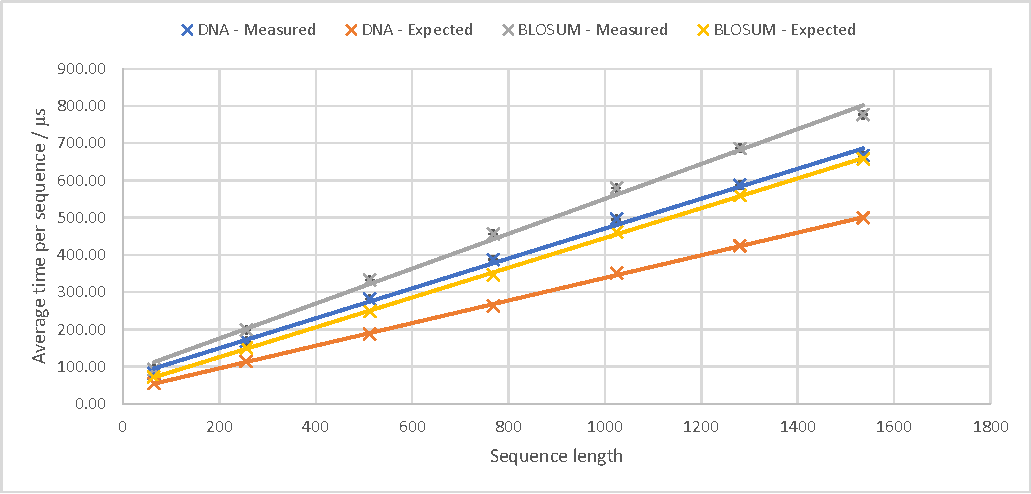
\includegraphics[width=\textwidth]{figs/eval/fpga_all.pdf}
    \caption{Modelled and actual latency of aligning two sequences of length $\SI{32768}{}$ against the given length, using a constant similarity function for DNA, and the BLOSUM50 scoring matrix for proteins. DNA: $R^2=0.9967$, BLOSUM: $R^2=0.9957$}
    \label{fig:FPGA_All}
\end{figure}

\subsubsection{Device utilisation}
\label{sec:FPGA_utilisation}

The utilisation statistics of different FPGA resources by designs help to quantify the limiting factors of the design; listed in \cref{tab:FPGA_Utilisation}.
The design aligning DNA sequences used a constant sequence similarity function, and the design aligning proteins used the BLOSUM50 lookup matrix.
Both designs use $98\%$ of the M10K blocks of RAM on the chip.
This is the limiting factor for the lengths of sequences that can be aligned, because the grid of alignment pointers are stored in block RAMs in my design.

The BLOSUM design has higher register and logic utilisation, due to the additional bits required to represent amino acids ($\SI{5}{\bits}$) rather than nucleotides ($\SI{2}{\bits}$) and the BLOSUM lookup matrix used by each processing element.
For both designs, the logic utilisation is enough to prevent the number of processing elements from being increased, as discussed in \cref{sec:Memory_in_SV}.
DSP blocks were not used, and the interconnect usage was low enough to not cause any issues.

\begin{table}
    \centering
    \begin{tabular}{|p{0.3\textwidth}|p{0.35\textwidth}p{0.35\textwidth}|} \hline
        Resource & Constant similarity DNA design & BLOSUM protein design \\ \hline
        Logic utilization (in ALMs) & $\SI{19784}{} \;/\; \SI{32070}{}$ ($62\%$) & $\SI{29635}{} \;/\; \SI{32070}{}$ ($92\%$) \\
        Total registers & $\SI{19149}{} \;/\; \SI{64140}{}$ ($30\%$) & $\SI{27405}{} \;/\; \SI{64140}{}$ ($43\%$) \\
        Total M10K Blocks & $391 \;/\; 397$ ($98\%$) & $39 \;/\; 397$ ($98\%$) \\
        Total DSP Blocks & $0 \;/\; 87$ & $0 \;/\; 87$ \\
        Average interconnect usage & $19.0\%$ & $29.0\%$ \\
        Peak interconnect usage & $38.5 \%$ & $44.5\%$ \\ \hline
    \end{tabular}
    \caption{Resource utilisation by the FPGA implementations}
    \label{tab:FPGA_Utilisation}
\end{table}

\begin{table}
    \centering
    \begin{tabular}{|l|ll|} \hline
        Design & PLL frequency  & Reported $F_{max}$ \\ \hline
        Constant similarity DNA & $\SI{79}{\mega\hertz}$ & $\SI{80.96}{\mega\hertz}$ \\
        BLOSUM Protein & $\SI{60}{\mega\hertz}$ & $\SI{60.99}{\mega\hertz}$ \\ \hline
    \end{tabular}
    \caption{Resource utilisation by the FPGA implementations}
    \label{tab:FPGA_Clocks}
\end{table}

\pagebreak

\Cref{fig:Chip_plan_base} shows the layout of FPGA resources used by the design aligning proteins using BLOSUM.
Logic elements are shown in blue, proportional to cell utilisation, and M10K blocks in green.
In \cref{fig:Chip_plan_array}, PEs in the systolic array are highlighted on a scale from white (start) to red (end).
The FIFO passing data between the last and first elements is shown in bright green, and the back-tracing unit in purple.
Some of the HPS-FPGA communication and logic is shown in yellow.
The other blue cells contain the logic and registers for retrieving and storing sequences received from the HPS.

\Cref{fig:Chip_plan_routing} shows routing utilisation.
The vertical striping is routing down columns of M10K blocks, and this is most congested around the M10K blocks that are used by but not near to the systolic array.
There is another routing hotspot around the interface pins between the FPGA and HPS.
However, none of these hotspots are congested enough to cause problems.


\subsubsection{Design clock speed}
\label{sec:SV_Fmax}

Using a Phase-locked loop (PLL), I was able to increase the clock speed of the design from the 50 MHz clock that is provided to the FPGA.
In \cref{tab:FPGA_Clocks} are the clock speeds used by my design, and the reported $F_{max}$ values for these designs.
Changing the PLL frequency changes the design as a whole and has an impact on the $F_{max}$ value reported.
The frequencies in \cref{tab:FPGA_Clocks} are based on the highest PLL frequencies I found which would result in the $F_{max}$ value being greater than the PLL frequency.
If the PLL frequency were to exceed the $F_{max}$ of the design, the design is likely to be unstable when instantiated on the FPGA.

\begin{figure}[H]
    \begin{subfigure}[b]{\linewidth}
    \centering
    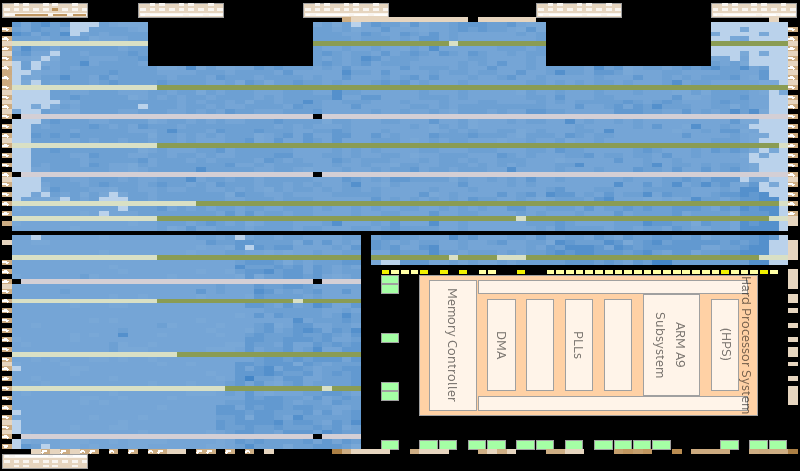
\includegraphics[width=0.72\linewidth]{figs/eval/base_chip_plan_cropped.png}
    \caption{Resources used: logic elements in blue (proportional to cell utilisation), M10K blocks in green}
    \label{fig:Chip_plan_base}
    \vspace{2ex}
    \end{subfigure}
    \begin{subfigure}[b]{\linewidth}
    \centering
    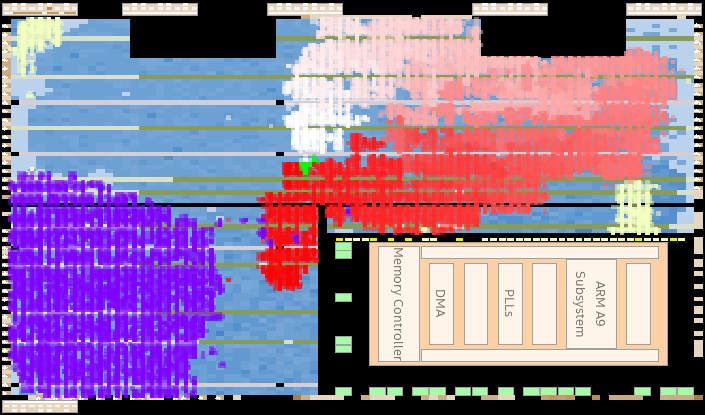
\includegraphics[width=0.72\linewidth]{figs/eval/pe_array_cropped.png}
    \caption{Different components of the design highlighted}
    \label{fig:Chip_plan_array}
    \vspace{2ex}
    \end{subfigure}
\begin{subfigure}[b]{\linewidth}
    \centering
    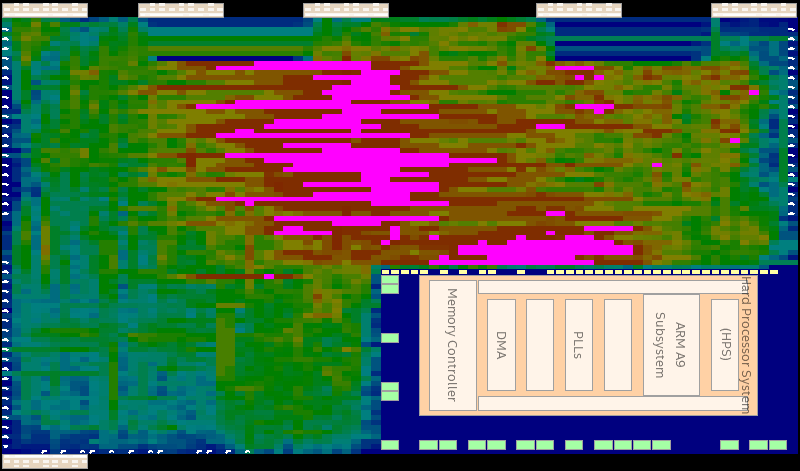
\includegraphics[width=0.72\linewidth]{figs/eval/routing_cropped.png}
    \caption{Routing utilisation, on a heatmap scale with pink for the peak areas}
    \label{fig:Chip_plan_routing}
    \vspace{2ex}
    \end{subfigure}
    \caption{FPGA chip layout of the design aligning proteins using BLOSUM}
    \label{fig:Chip_plans}
\end{figure}



% !TeX root = ../diss.tex

\chapter{Conclusions}

In conclusion, this project was successful.
The core criteria, producing single and multi-threaded C, and CUDA implementations of the Smith-Waterman algorithm, were achieved.
As was one of the extensions, to implement and instantiate the algorithm on an FPGA.
Investigations into the impact of different ways of scoring alignments were performed, and the performance of the different implementations were compared.

\section{Results}
\label{sec:Concl_results}

As I initially suspected, the Smith-Waterman algorithm was amenable to parallelisation, with the GPU implementation outperforming the CPU implementation for large sequences.
However, smaller alignments have less scope for parallelisation, and the CPU could outperform the GPU with better sequential performance.

I only had time to make an implementation for the FPGA that could align short sequences.
The accelerator I designed was highly specialised and was able to do a lot of work each clock cycle, albeit at a modest clock speed.
For these short sequences, it outperformed the CPU and GPU implementations by a significant margin.

\section{Further work}
\label{sec:Concl_further work}

I cannot think of any major insufficiencies in the C and CUDA implementations I made.
Undoubtedly improvements could be made by hand-optimising the assembly code, but I suspect this would not yield major improvements.
An extension which I did not have time for was to modify my C implementation to use the Streaming SIMD Extensions of the x86 platform to improve the performance of my CPU-based implementation, and this could be investigated.

However, the FPGA implementation was ambitious and has obvious areas for improvement.
Alone it could have been the basis for a whole Part II Project, but using good planning I used the time I had to produce a limited design that could align sequences.
Two areas of improvement are:
\begin{itemize}
\item Modifying the design to align much longer sequences, using the linear space approach (\cref{sec:SW_Linear_Prep}).
This would require the original, quadratic space implementation to perform the alignments of sufficiently small subproblems.
Either a larger FPGA could be used where both designs could be instantiated together, or perhaps they could be combined where the accelerator chooses its alignment algorithm based on sequence length.

\item Improving the clock speed of the design through pipelining.
The critical paths in my design were inside of processing elements, performing long sequences of arithmetic and comparisons each clock cycle.
This arithmetic could be divided into pipeline stages, allowing the clock to run at a higher frequency.

\end{itemize}


%%%%%%%%%%%%%%%%%%%%%%%%%%%%%%%%%%%%%%%%%%%%%%%%%%%%%%%%%%%%%%%%%%%%%
% the bibliography

\addcontentsline{toc}{chapter}{Bibliography}
\printbibliography[heading=secbib]

%%%%%%%%%%%%%%%%%%%%%%%%%%%%%%%%%%%%%%%%%%%%%%%%%%%%%%%%%%%%%%%%%%%%%
% the appendices
\appendix

% \chapter{Repository overview}
% \label{sec:Repo_overview_app}

% % !TeX root = ./diss.tex

\DTsetlength{0.2em}{1em}{0.2em}{1pt}{4pt}
\begin{figure}[H]
\dirtree{%
    .1 /.
    .2 cpu\_code\DTcomment{C implementation}.
        .3 correctness\_tester.c \DTcomment{Basis for correctness testing across implementations}.
        .3 helpers.c \DTcomment{Utility functions}.
        .3 main.c \DTcomment{Entry point; rudimentary command line interface}.
        .3 nw.c \DTcomment{Initial global alignment implementation}.
        .3 sw.c \DTcomment{Local alignment implementation, quadratic and linear space}.
        .3 swParallel.c \DTcomment{Multi-threaded local alignment implementation}.
        .3 swGotoh.c \DTcomment{Affine gap implementation, quadratic and linear space}.
        .3 swGotohParallel.c \DTcomment{Multi-threaded affine gap alignment implementation}.
    .2 gpu\_code\DTcomment{CUDA implementation}.
        .3 helpers.cu \DTcomment{Utility functions}.
        .3 main.cu \DTcomment{Entry point; rudimentary command line interface}.
        .3 sw.cu  \DTcomment{Local alignment implementation, quadratic and linear space}.
        .3 swSingleBlock.cu \DTcomment{Quadratic space local alignment, without block-parallelism}.
        .3 swGotoh.cu \DTcomment{Affine gap implementation}.
    .2 fpga\_code\DTcomment{FPGA implementation}.
        .3 c\_interface \DTcomment{C Interface for ARM HPS}.
            .4 sequence\_reader.c \DTcomment{Reading sequences from files}.
            .4 start.c \DTcomment{Interface with FPGA}.
        .3 systemverilog \DTcomment{SystemVerilog implementation}.
            .4 datatypesPkg.sv \DTcomment{Types of signals used}.
            .4 macro.vh \DTcomment{Implementation-wide macros to change types of sequences}.
            .4 pe\_bram.v \DTcomment{BRAM for grid of pointers}.
            .4 fifo\_16b\_1024w.v \DTcomment{BRAM FIFO for storing previous column of scores}.
            .4 backtrace.sv \DTcomment{Backtracing through a grid of registers}.
            .4 backtrace\_with\_ram.sv \DTcomment{Backtracing through a grid in M10K BRAM}.
            .4 pe.sv \DTcomment{Single processing element where pointer grid is registers}.
            .4 pe\_with\_ram.sv \DTcomment{Single processing element where pointer grid is BRAM}.
            .4 short\_solver.sv \DTcomment{Systolic array for sequences the length of the array}.
            .4 short\_solver\_avalon.sv \DTcomment{Avalon FPGA-HPS interface for \lstinline{short_solver}}.
            .4 med\_solver.sv \DTcomment{Systolic array for sequences of lengths $1024 \times 1536$}.
            .4 med\_solver\_with\_ram.sv \DTcomment{\lstinline{med_solver} but using BRAM for pointer grid}.
            .4 med\_solver\_with\_ram\_avalon.sv \DTcomment{Main Avalon FPGA-HPS interface}.
            .4 tb\_blosum.sv \DTcomment{Various testbenches (\lstinline{tb_*})}.
            .4 tb\_med\_solver.sv .
            .4 tb\_med\_solver\_with\_ram.sv .
            .4 tb\_pe.sv .
            .4 tb\_short\_seq.sv .
            .4 tb\_short\_solver.sv .
        .3 quartus \DTcomment{Configuration files from my Quartus Lite project}.
}
\caption{Header files (of extensions \lstinline{.h} and \lstinline{.cuh}) have been omitted from for brevity, and always correspond to a code file. Makefiles have also been omitted.}
\label{fig:Repo_tree}
\end{figure}


\chapter{Project Proposal}
\label{sec:Proposal}

% !TeX root = ./proposal.tex

% Draft #1 (final?)

\centerline{\Large Computer Science Tripos -- Part II -- Project Proposal}
\vspace{0.4in}
\centerline{\Huge Parallelising Sequence Alignment}
\vspace{0.4in}
\centerline{\large \candidate, Sidney Sussex College}
\vspace{0.1in}
\centerline{\large Originator: Mr P. Rugg}
\vspace{0.1in}
\centerline{\large 25 October 2019}
\vspace{0.5in}

\noindent
{\bf Project Supervisor:} Mr P.~Rugg

\noindent
{\bf Director of Studies:} Mr M. Ireland

\noindent
{\bf Project Overseers:} Prof~J. Daugman  \& Dr~A. Madhavapeddy

% Main document

\section*{Introduction}

Sequence alignment is an important tool in Bioinformatics, used to find relationships between sequences of DNA, RNA, or proteins.
The molecules in question are long polymers, made up of a sequence of different much smaller molecules.
In DNA and RNA, there are four possible monomers called nucleotides, and in proteins there are twenty naturally occurring monomers called amino acids.
Pairwise sequence alignment involves taking two sequences of monomers, and determining which monomers in each sequence correspond to one another and where monomers must have been inserted or deleted.

This is a valuable tool for Bioinformaticians, and finding sequence alignments is a computationally challenging problem.
The different biological meanings of different types of sequence can be simplified into two sequences of characters, with some kind of scoring function to evaluate the quality of the alignment.
Find an optimal alignment is often solved using a dynamic programming approach, building up possible alignments in a grid and the alignment with the best score is chosen when the grid as been populated.
This is the Smith-Waterman algorithm.
When evaluated sequentially, the execution time is $O(nm)$ where $n$ and $m$ are the lengths of the two strings.
However, as the grid is populated the number of cells available to be evaluated grows, so the potential to parallelise execution grows as execution proceeds.
This can reduce execution time to $O(n)$, provided that there is sufficient hardware to run $m$ threads parallel to one another.

This project aims to explore the differences between hardware architectures such as general purpose processors and graphics processing units, and as an extension FPGAs.
Graphics processing units are capable of evaluating hundreds of instructions simultaneously, which I expect will give it a significant advantage over general purpose processing units.
I expect an FPGA will prove to be an interesting platform to investigate, because of the potential to be able to make all of the calculations and decisions for a cell in the dynamic programming grid, in a single clock cycle.
The hardware logic on an FPGA can be focussed on a single problem, unlike other platforms like GPUs where there will logic not being used by my software, which should allow the FPGA to consume less power.

I will produce software or hardware logic that find sequence alignments, and then compare the different implementations using metrics such as time taken to find alignments, electrical power usage and hardware costs.

\section*{Starting Point}

I have pre-read the relevant sections of the Bioinformatics course (and those lectures will have been delivered by the end of the October), so I understand the basic algorithms underpinning sequence alignment.
I have previous experience writing C code from the Programming in C and C++ course from Part IB, and wrote some during a summer internship as well.
I have very little experience using GPU APIs such as CUDA, having written a very small amount of GLSL in the Introduction to Graphics course, so I will need to learn how to use CUDA as part of this project.
During the ECAD and Architecture course I worked with an FPGA, and have written SystemVerilog as a part of that course, though I have no experience with FPGAs beyond that course.

I have read a few papers about parallelising sequence alignment, and it is worth noting that a similar project was undertaken by Benkrid et al. in 2012 \cite{Benkrid12}.
However, their work is several years old and different conclusions might be drawn when using more modern hardware, as I intend to do.
Additionally, I intend to evaluate performance more thoroughly, and investigate factors that may have an impact on that performance, such as alignment metrics or the impact of different compilers.

\section*{Work to be done}

The implementation phase of the project breaks down into the following sections:

\begin{enumerate}

\item Implementing the Smith-Waterman algorithm to find sequence alignments using single-threaded C code.

\item Modifying the C code to make it multi-threaded.

\item Implementing the Smith-Waterman algorithm using CUDA to run on a GPU.

\end{enumerate}

\section*{Extensions}

My primary extension will be to implement the Smith-Waterman algorithm on an FPGA, and I hope to complete this extension.
However, it is not a primary goal because of my unfamiliarity with FPGAs having only done ECAD and Architecture labs, and this will be much more complicated than anything I have attempted to implement on an FPGA before.

Another extension is to modify my C implementation to use vectorised instructions, exploiting SIMD parallelism in a similar way to my CUDA implementation.

\section*{Success criteria \& Evaluation}

The goal of this project is to compare the effectiveness of different computer processing technologies, particularly focussing on producing parallelised implementations.
This focus on parallelism is to make the project relevant to modern machines, because GPUs are designed to perform hundreds of operations concurrently and modern CPUs all have multiple cores.
This is in part due to Moore's Law slowing down, and parallelism is increasingly becoming the approach used to increase the performance of computers instead of shrinking silicon process nodes.

My success criteria are to produce implementations of the Smith-Waterman algorithm in single-threaded C, multi-threaded C, and CUDA, and to thoroughly evaluate their performance.
This will involve finding how the time it takes to find sequence alignments changes for different lengths of sequences, and comparing the performance to approximate power usage.
If I produce an implementation to be run on an FPGA, I plan to evaluate that in a similar fashion.
For all of the solutions I implement, I intend to implement a variety of alignment-scoring functions (simple edit distance, different gap penalties, substitution matrices such as BLOSUM, etc.), and compare the performance impact that these different functions can have on these different platforms.
As extensions to the evaluation, I could investigate the impact of using different compilers and optimisation modes has on the runtime of my solutions.

\section*{Work Plan}

As a student taking CST Part II 50\% taking a similar number of Paper 8 and 9 courses in Michaelmas and Lent terms, I have a consistent lecture load throughout the year with no particularly quiet nor intense periods which students taking Part II Units of Assessment might experience.
Therefore, I will not be accounting for differences in lecture load in my timetable.
However, I am taking three papers at the end of the year so I intend to have handed in by dissertation by 24th April (in Week 1 of Easter term), giving me the whole term to focus on my last lecture series and revision.

\subsection*{14th Oct -- 27th Oct}
Write my proposal, with a draft handed in on 18th Oct and the final version handed in by 25th Oct.
General project setup such as installing compilers, setting up version control arrangements, sorting out \LaTeX\ typesetting for my proposal and dissertation.

\textit{Milestone}: Final Proposal submitted.

\subsection*{28th Oct -- 10th Nov}
Implement Smith-Waterman algorithm as single-threaded C program, and find a subset of protein sequences from UniProt \cite{UniProt} for testing.
These will be used to evaluate the correctness of all of the subsequent implementations I make.

\nopagebreak
\textit{Milestone}: Single threaded C program written, with tests for correctness.

\subsection*{11th Nov -- 24th Nov}
Modify the single-threaded C to run using multiple threads. Begin writing the Preparation chapter of my dissertation.

\textit{Milestone}: Multi-threaded C program written, tested for correctness.

\subsection*{25th Nov -- 8th Dec}
Write a basic CUDA implementation of the Smith-Waterman algorithm. Continue writing the Preparation chapter of my dissertation.

\textit{Milestone}: Basic CUDA implementation, tested for correctness.

\subsection*{8th Dec -- 21st Dec}
Improve my CUDA implementation of the Smith-Waterman algorithm, considering branches and memory layouts.
Finish first draft of the Preparation chapter.
I doubt this will take the full two weeks, but it provides some space to catch up if things have slipped behind.
If this is not necessary, I can begin work on the next milestone.

\textit{Milestone}: Finished CUDA implementation, finished Preparation chapter draft.

\subsection*{6th Jan -- 19th Jan}

These slots are dedicated to extensions, but would also serve as slack time if things are running behind from the beginning of the project.
Start with adding vectorised CPU instructions to my C code (which should require a similar approach to my CUDA application).
After that, begin work on the FPGA extension: design logic to find small sequence alignments, small enough that the problem doesn't need to be split into subproblems.
Sequences will be hard coded instead of taking them from an external source such as the ARM CPU on the same chip as the FPGA.
This logic only needs to be simulated for this milestone. Begin work on progress report.

\textit{Milestone}: Basic FPGA implementation made and testing in simulation.

\subsection*{20th Jan -- 2nd Feb}

Finish and rehearse progress report.
\nopagebreak
Continue work on FPGA extension: Work on synthesising logic and running it on the FPGA.
Add the ability to for the ARM core on the same chip to deploy and collect work from the FPGA, using it as a hardware accelerator.

\nopagebreak
Assess at the end of this block how well the FPGA extension is going, and whether to continue with it.

\nopagebreak
\textit{Milestone}: Hand in progress report. Synthesise logic from last milestone and run on the FPGA. Sort out the interface between ARM core and FPGA on the development board.

\subsection*{3rd Feb -- 16th Feb}

Work on the ability to divide up sequences on the FPGA so sequences of arbitrary length can be aligned, using a scaled down model in simulation.
At the end of this work package, stop work on extensions regardless of their progress to focus on writing my dissertation.

\textit{Milestone}: Deliver progress report. Implementation phase of project complete.

\subsection*{17th Feb -- 1st Mar}

Begin writing implementation chapter of my dissertation, and start evaluating my work.
The range of test-sequence lengths required should be apparent from the approximate performance observed when testing the implementations.
I will consult other papers to decide on lengths of test sequences that might represent a real-world work load as well, to add context to my results.

\textit{Milestone}: Numerical evaluation of C code complete.

\subsection*{2nd Mar -- 15th Mar}

Finish writing draft of implementation chapter of my dissertation, and finish numerical evaluation. Begin writing Evaluation chapter.

\textit{Milestone}: Implementation chapter drafted. Numerical evaluation of CUDA code (and FPGA logic if it is working) complete

\subsection*{16th Mar -- 29th Mar}

Finish writing the Evaluation chapter, and write Introduction and Conclusion chapters.
Work on any feedback on my dissertation I receive.

\textit{Milestone}: Introduction, Conclusion, and Evaluation chapters drafted.

\subsection*{30th Mar -- 12th Apr}

Finish any writing that may have slipped behind, and submit a draft to my supervisor and Director of Studies for feedback.

\textit{Milestone}: None

\subsection*{13th Apr -- 26th Apr}

Final work based on feedback, then submit dissertation.

\textit{Milestone}: Dissertation submitted.

\section*{Resources}

I plan to use my own laptop for this project. It has a hexa-core CPU (an Intel i7-8750H), 16 GB RAM, 512 GB SSD and an NVIDIA GTX 1050 Ti Max-Q graphics chip, running Windows 10.
I accept full responsibility for this machine and I have made contingency plans
to protect myself against hardware and/or software failure.

All work towards the project and dissertation will be held under Git with a copy hosted on Github, and any work done each day will be pushed to this repository.
Onedrive will also be used for real-time file mirroring, meaning I won't depend
on a single cloud service.

In the event that I won't be able to use my laptop, I have an old laptop (dual-core CPU, 8 GB RAM, integrated Intel graphics chip) to use for development and writing, and I could use MCS machines as well.
I will be able to pull my work from the cloud and continue working with minimal disruption.

Computationally difficult experiments may be slow on these devices, so the Computer Architecture group has agreed to provide me with access to a machine to evaluate my C implementation on.

Another important resource the Computer Architecture group has agreed to provide me with is an access to an FPGA.
This is only required for an extension to the project, but time allowing it is something I would like to attempt.
The DE1-SoC boards used in ECAD+Arch labs by Part IB students are ideal, with relatively small FPGA chips so I will be able synthesise my work on my laptop in reasonable periods of time.


\end{document}
